\documentclass[a4paper,11pt,final]{article}
% Pour une impression recto verso, utilisez plutôt ce documentclass :
%\documentclass[a4paper,11pt,twoside,final]{article}

\usepackage[english]{babel}
\usepackage[utf8]{inputenc}
\usepackage[T1]{fontenc}
\usepackage[pdftex]{graphicx}
\usepackage{setspace}
\usepackage{hyperref}
\usepackage[french]{varioref}

\newcommand{\reporttitle}{Exemple de rapport}     % Titre
\newcommand{\reportauthor}{Bruno \textsc{Voisin}} % Auteur
\newcommand{\reportsubject}{Stage de fin d'étude} % Sujet
\newcommand{\HRule}{\rule{\linewidth}{0.5mm}}
\setlength{\parskip}{1ex} % Espace entre les paragraphes

\hypersetup{
    pdftitle={\reporttitle},%
    pdfauthor={\reportauthor},%
    pdfsubject={\reportsubject},%
    pdfkeywords={rapport} {vos} {mots} {clés}
}
\usepackage{balance}

%% to enable \thank command

%% The usage of the following packages is recommended
%% to insert graphics
\usepackage{graphicx}
% to typeset algorithms
%\usepackage{algorithmic}
\usepackage{algorithm}
% to typeset code fragments
\usepackage{listings}
% to make an accent \k be available
\usepackage[OT4,T1]{fontenc}
% provides various features to facilitate writing math formulas and to improve the typographical quality of their output.
\usepackage[cmex10]{amsmath}
\interdisplaylinepenalty=2500
% por urls typesetting and breaking
\usepackage{url}
% for vertical merging table cells
\usepackage{amsthm}
\usepackage{multirow}
\theoremstyle{definition}
\newtheorem{definition}{Definition}[section]

\usepackage{filecontents}

\usepackage{booktabs}% http://ctan.org/pkg/booktabs
\newcommand{\tabitem}{~~\llap{\textbullet}~~}

\usepackage{color}
\usepackage{xcolor}
\usepackage{colortbl}
\definecolor{LightCyan}{rgb}{0.88,1,1}
\definecolor{BluishGray}{RGB}{226,227,231}
\definecolor{LightGray}{gray}{0.95}
\definecolor{Gray}{gray}{0.85}
\usepackage{algpseudocode,algorithmicx}
\usepackage{comment}
\newcommand*\DNA{\textsc{dna}}

\newcommand*\Let[2]{\State #1 $\gets$ #2}
\algrenewcommand\algorithmicrequire{\textbf{Input:}}
\algrenewcommand\algorithmicensure{\textbf{Output:}}
\algrenewcommand\algorithmicrequire{\textbf{Input:}}
\algrenewcommand\algorithmicensure{\textbf{Output:}}

% define environments for remarks and examples
\newtheorem{remark}{Remark}[section]
\newtheorem{example}[remark]{Example}
\newcommand{\ti}{\textit}
\newcommand{\tb}{\textbf}

\setlength{\textfloatsep}{1\baselineskip plus 0.2\baselineskip minus 0.8\baselineskip}
\lstset{
	language=Ada,                % choose the language of the code
	basicstyle=\tiny,       % the size of the fonts that are used for the code
	%numbers=left,                   % where to put the line-numbers
	%numberstyle=\footnotesize,      % the size of the fonts that are used for the line-numbers
	%stepnumber=1,                   % the step between two line-numbers. If it is 1 each line will be numbered
	%numbersep=5pt,                  % how far the line-numbers are from the code
	backgroundcolor=\color{white},  % choose the background color. You must add \usepackage{color}
	showspaces=false,               % show spaces adding particular underscores
	showstringspaces=false,         % underline spaces within strings
	showtabs=false,                 % show tabs within strings adding particular underscores
	%frame=single,           % adds a frame around the code
	tabsize=2,          % sets default tabsize to 2 spaces
	captionpos=b,           % sets the caption-position to bottom
	breaklines=true,        % sets automatic line breaking
	breakatwhitespace=false,    % sets if automatic breaks should only happen at whitespace
	escapeinside={\%*}{*)},          % if you want to add a comment within your code
	numbers=right,
	numbersep=-10pt,
	numberstyle=\tiny,
}


%
%
\title{Rapport}
%
%


% conference papers do not typically use \thanks and this command
% is locked out in conference mode. If really needed, such as for
% the acknowledgment of grants, issue a \IEEEoverridecommandlockouts
% after \documentclass

% for over three affiliations, or if they all won't fit within the width
% of the page, use this alternative format:
% 
%\author{\IEEEauthorblockN{Michael Shell\IEEEauthorrefmark{1},
%Homer Simpson\IEEEauthorrefmark{2},
%James Kirk\IEEEauthorrefmark{3}, 
%Montgomery Scott\IEEEauthorrefmark{3} and
%Eldon Tyrell\IEEEauthorrefmark{4}}
%\IEEEauthorblockA{\IEEEauthorrefmark{1}School of Electrical and Computer Engineering\\
%Georgia Institute of Technology,
%Atlanta, Georgia 30332--0250\\ Email: see http://www.michaelshell.org/contact.html}
%\IEEEauthorblockA{\IEEEauthorrefmark{2}Twentieth Century Fox, Springfield, USA\\
%Email: homer@thesimpsons.com}
%\IEEEauthorblockA{\IEEEauthorrefmark{3}Starfleet Academy, San Francisco, California 96678-2391\\
%Telephone: (800) 555--1212, Fax: (888) 555--1212}
%\IEEEauthorblockA{\IEEEauthorrefmark{4}Tyrell Inc., 123 Replicant Street, Los Angeles, California 90210--4321}}





\begin{document}
  \maketitle              % typeset the title of the contribution
  \cleardoublepage % Dans le cas du recto verso, ajoute une page blanche si besoin
  \tableofcontents % Table des matières
  \sloppy          % Justification moins stricte : des mots ne dépasseront pas des paragraphes
  \cleardoublepage
  \include{remerciements}
  \begin{abstract}
%Model-Driven Engineering (MDE) is a development paradigm that brings the benefits of increased automation to the software development cycle.
%The MDE community tries to promote MDE adoption by pushing models written in diagram-based languages, supported by extensive tooling.
%While there is increasing evidence that MDE facilitates the design of complex software, its level of acceptance by software developers is still low.
%On one hand, rather than use diagram-based languages, most programmers prefer to work with their favorite text-based languages (e.g. Java and C++)
%and integrated development environment.
%On the other hand, software architects are among the early adopters and promoters of diagram-based languages.
%They consider such languages to be much more suitable for describing architectures compared to textual languages.
%Synchronizing manually written artifacts in either type of language is not simple and is often very time-consuming and error prone unless it is supported
%by automated methods and tools.

%To solve this issue, we propose a methodological pattern for model-code synchronization supported by corresponding tooling. 
%The solution tackles a fundamental problem of round-trip engineering: synchronization between concurrently evolving artifacts. 
%On one side we have the architecture model maintained by the software architects, while on the other, we have code written by programmers.
%Applying our approach for the development of an actual runtime system, we show that both parties involved, software architects and programmers, can efficiently collaborate while continuing to work in their favorite development environment.
\end{abstract}

  \cleardoublepage
  %TODO introduce notion of viewpoint consistency and say that it is an important part of what we propose and why we propose it
%TODO reinforce notion of collaboration between software architects and programmers, that is a motivation of our work
\section{Introduction}
\label{sec:introduction}

% What is MDE and how are models seen by the MDE community who creates a gap between modeling and coding
Internet of Things \cite{Li2015} raises the complexity of embedded systems today rapidly. 
Model-Driven Engineering (MDE) is recognized as an efficient means to deal with the complexity.
MDE \cite{selic_what_2012} promotes abstraction and automation. 
The latter often relies on chaining transformations from source models at high level abstraction to target models and finally to code. 
Those two techniques are identified as model to model (M2M) and model to code (M2C) transformations.
%Traditionally, the MDE community draws a sharp distinction between development
%using a diagram-based language (commonly called a modeling language in the MODELS \cite{models_conf} community)
%and development using a textual language (i.e. a programming language or code). 
Among modeling languages, the Unified Modeling Language (UML) is most widely used. 
UML and its diagrams are much more useful to design such systems than text-based languages. 
Especially, in embedded system domains such as vehicle controlling, UML State Machines \cite{Cruz-Lemus2005} are used as a powerful means to describe the dynamic behavior of such complex systems.

%Proponents of MDE have argued that adopting model-centric approaches
%would benefit software developers due to its many advantages
%\cite{selic_what_2012}, especially for development of complex systems.
%They encourage the greater use of model-driven development,
%by, among other initiatives, providing diagram-based languages
%supported by appropriate tools \cite{gerard_once_2015}
%such as automated code generation.

% Problem: perceived difference between diagram-based language and textual language
%In industrial practice, there is still significant reticence to adopt a
%fully model-centric approach \cite{hutchinson_model-driven_2011, selic_what_2012}.

%This is all the more true
%for models that are described in diagrams \cite{brown_position_2015}.
Ideally, a full model-centric approach is preferred by the MDE community due to its advantages \cite{selic_what_2012}. However, in industrial practice, there is significant reticence \cite{Hutchinson:2011:MEP:1985793.1985882} to adopt it. 
The reticence is due in part to
the perceived gap \cite{brown_position_2015} between diagram-based languages
and textual languages.
On one hand, programmers prefer to
use the more familiar textual programming language. 
On the other hand, software architects, working at higher levels
of abstraction, tend to favor the use of models, and therefore
prefer graphical languages for describing the architecture of
the system (see Fig. \ref{fig:inconsistency}).

The survey described in \cite{hutchinson_model-driven_2014,Forward2008} polled stakeholders in companies
who use MDE approaches. 
The survey reveals that UML is the prominent and dominating language. 
85\% of the respondents used UML for various purposes, especially problem understanding and automation such as code generation (88,2\%). 
It notes that 70\% of the respondents primarily work
with models, but still require manually-written code to be integrated.
Furthermore, 35\% of
the respondents answered that they spend a lot of time and effort synchronizing
model and code. The need of synchronization is critically required by systems today. 
Besides the synchronization aspect, efficiency of code generated from models is a concern for the respondents. 

%Yet, still in another survey \cite{Forward2008}, the authors compare code-centric and model-centric approaches by asking the participants, who mostly come from Canada, United States and other countries such as United Kingdom, France, Indian, Australia and Singapore, questions related to different activities in software development such as fixing a bug, creating efficient software and a system as quickly as possible. 
%The results shows that most activities tend to be easier in a model-centric approach but many participants believe that a code-centric approach is much easier a model-centric approach.
%This confirms the importance of automatically keeping model and code synchronized.
      

The code modified by programmers and the model are then inconsistent. 
Round-trip engineering (RTE) \cite{Hettel2008} achieves synchronization between related artifacts
that may evolve concurrently by incrementally updating each artifact
to reflect editions made in the other artifacts.
RTE enables actors (software architect and programmers) to freely move between different representations \cite{Sendall} and stay efficient with their favorite working environment. 

Even, if the code is not intended to be modified by programmers, RTE is still helpful in the state-of-the-art MDE practice, e.g. debugging generated code. Some code generators generate fully operational code. The debugging support helps developers trace bugs in the generated code back to precise model elements. 

% Problem: even in MDD, as described by the MDE community, code is not entirely moved out
%Even in teams who embrace a model-driven approach,
%the gap between model and code is not bridged seamlessly.

The back-and-forth switching between diagram-based and textual languages, as well as
between model and code,
%along with the effort necessary for artifacts synchronization,
has hindered the adoption of MDE in industrial practice.
To solve this issue, we believe that the sharp distinction between model and code must be blurred.
We feel that a collaborative solution must be offered to
different categories of developers (e.g. architects, programmers),
who use different development practices.
%The solution must not impose a choice between a diagram-based language and a textual language.


\begin{figure}
	\centering
	\includegraphics[trim={4.5cm 6.6cm 5cm 3cm},clip, width=0.8\columnwidth]{figures/inconsistency}
	\caption{Concurrent modifications made to different artifacts}
	\label{fig:inconsistency}
\end{figure}

Collaboration between developers producing different types of artifacts, in different languages,
using different tools,
raises the issue of artifact synchronization.
This is a well-known concern with round-trip engineering \cite{sendall_taming_2004}.
%Namely, round-trip engineering requires the ability to maintain consistency
%between multiple concurrently evolving software artifacts \cite{sendall_taming_2004}.
It is related to traditional software engineering disciplines
such as forward
and reverse engineering \cite{chikofsky_reverse_1990}.



Usually, a direct synchronizing between the architecture model and the code is hard because of the large abstraction gap. The synchronization is therefore decoupled into several synchronization steps of artifacts participating in one of the transformation phases of the chain. Hence, the whole synchronization is achieved if these steps do. 

\subsection{Research method}
The research is realized by an iterative method depicted in Fig. \ref{fig:researchmethod}.
We started by studying the literature related to MDE and approaches to integrating MDE into industrial practice. 
We are interested in approaches for developing embedded systems using synchronization of model and generated code, which is critical as previously discussed.
Specifically, we found that, (1) current approaches and tools do not support synchronization of concurrent modifications made to model and code. Furthermore, (2) the synchronization is, for UML community, only supported for available concepts of UML class diagrams while the behavior model such as UML State Machine (USM) is not supported.
The reason is that there is no trivial mapping between mainstream programming languages such as C++ and Java, and the behavior model.

However, USM plays an important role in modeling and designing reactive, real-time, embedded systems.
Hence, the lack of synchronization support for USMs harms enterprises to adopt UML as a development language.
%It is how our motivation is established.


It is common in MDE that code is generated, from either USMs or component models, by using templates.
When models or templates change, code needs to be changed accordingly.
However, when these artifacts are concurrently modified, for some reasons, making these consistent again are challenging. 
Some approaches using specialized comments such as \ti{@generated} and \ti{@non generated} to specify which code areas should be untouched or modified, respectively.
By this way, when model elements and code change, code areas (user-modified code) marked by \ti{@non generated} are preserved. 
It means that changes made to models or templates are not propagated to some code areas. 
This may lead to the dead code problem, in which the user-modified code is not used in the new generated code (see \ref{subsec:sync-template} for more details).
Hence, we realize (3) the problem of models, code, and template co-evolution, which is not solved by existing approaches.

Once these related problems are identified, we then focus on defining and resolving the problems by proposing different approaches, whose goal to gain the acceptance of MDE by the enterprises.
The development and evaluation of the solutions are then conducted.
We iteratively evaluate by going to results of evaluation, compare with other approaches, and check whether the solutions can be improved to get better results.
%Once

\begin{figure}[b]
	\centering
	\includegraphics[trim={1.0cm 0.2cm 2.0cm 7.3cm},clip, width=1.04\columnwidth]{figures/researchmethod}
	\caption{Research method}
	\label{fig:researchmethod}
\end{figure}

\subsection{Major topics}
\label{subsec:majors}
To sum up, the thesis can be divided into two related major parts as followings:
\begin{itemize}
	\item \tb{Artifact synchronization}: As previously discussed, this is critical for step-by-step integrating MDE into current software development practices and collaborating these with MDE methodologies. Particularly, synchronization of artifacts is realized by means of incremental model-to-model and model-to-text transformations. Architecture models are often at a higher level abstraction than low level implementation code. Mappings from the architecture are usually not one-to-one. This raises the difficulty in mapping code-side elements back to architecture model-side elements. The existing synchronizations (state of the art) mainly focus on static parts while the dynamics are missing.
	
	\item \tb{Improving code generation solutions and towards synchronization for UML State Machine}: UML State Machines are widely used for reactive, real-time and embedded systems. However, the synchronization between UML State Machine and generated code is not supported by any existing approaches, even though it is critical. 
	Furthermore, on the one hand, the OMG seeks to raise the usefulness of UML State Machine by providing more modeling concepts supporting software architects for modeling and designing complex systems. 
	On the other hand, the support of existing generation approaches, over the years of research and development, is still limited to simple cases, especially when considering concurrency, pseudo state and event support. 
	
	\item \tb{Co-evolution of models, code, and generation templates}.  
	
	%\item \tb{Model-code co-debugging (MCCD)}:	Debugging is one of the most important activities in software development to find and fix bugs. 
	%In MDE, when having bugs in generated code, it is difficult to locate the code statements or the model elements, which have the bugs. 
	%MCCD enables modelers/developers to set breakpoints on model elements/code statements, respectively, and the breakpoints are also set on the associated code elements/model elements.
	%Thus, MCCD helps seamlessly collaborate model and code in debugging.
	%Current tools and approaches \cite{moka} support the model execution and debugging, especially for UML Activity and State Machine Diagrams, using Java/fUML as underlying action language.
	%However, model-code co-debugging 	 
\end{itemize}

\begin{comment}
In reality, UML State Machine might be used for different use-cases, either with RTE or not. 
We consider the second topic in different use-cases. Fig. \ref{fig:smapproaches} shows three cases. 
There are trade-offs between these. In the use-case (a), code generators can generate efficient code from state machines with full features (this is detailed in this report).
The case (b) (see \ref{subsec:usm2code}) only supports a small sub-set of modeling features and trades a reversible mapping with a memory overhead. 
The case (c) is a harmonization of the other two but restricts developers to a domain specific language (DSL). 

\begin{figure}
	\centering
	\includegraphics[trim={5.4cm 8.1cm 11.6cm 4.2cm},clip, width=0.8\columnwidth]{figures/smapproaches}
	\caption{Different usages of UML State Machine code generators and RTE: (a) state machines are generated to code and modifications only made to the state machines; (b) code generated from state machines is modified and synchronized directly with the state machines; and (c) generated code is modified indirectly via a text-based domain specific language (DSL).}
	\label{fig:smapproaches}
\end{figure}


\subsection{Problem statement}
\begin{itemize}
	\item Architecture models are often at higher level abstraction than low level implementation code. Mappings from the architecture are usually not one-to-one. This raises the difficulty in mapping code-side elements back to architecture model-side elements. The existing synchronizations mainly focus on static parts while the dynamics are missing.
	
	\item While UML State Machine are a powerful means to modeling the logical behavior of complex systems, the support for generating code from state machines and the efficiency of the generated code are limited to non-concurrency with issues such as memory consumption and processing speed. 
\end{itemize}
\end{comment}

\subsection{Objective}
The transformation from architecture models to code directly involves chaining model-to-model and model-to-text transformations. Therefore, to synchronize the architecture models and code, the following objectives need to be met:
\begin{itemize}
	\item A generic methodology, which synchronizes two different system artifacts (model and code). This method is based on incremental model transformation and synchronization. It will be used in different specific synchronization cases developed in the thesis deployment.
	
	\item A specific synchronization between UML State Machine with full features and code. %This will gain the usage of MDE in software development today. 
	Therefore, one task is needed to 
	%seamlessly make the behavior of the code generated from UML State Machine complied with the semantics specified by the Precise Semantics of UML State Machine (PSSM) \cite{OMG2015}. 
	%To do it, the objective of this part is to 
	provide a complete generation solution, especially considering the concurrency support for real-time systems. From the generation solution, a specific synchronization methodology combined with the generic one as above is also desired.  
	
	\item Synchronization of and making concurrently modified models, code, and templates consistent again.    
\end{itemize}

The final goal is to provide a common framework with many facilities for collaborating MDE developers and programmers so effectively that the acceptance of MDE in practice can be gained.

\subsection{Contributions}
The contributions of this report are the followings:
\begin{itemize}	
	\item An extensible generic methodology, which synchronize two different system artifacts (model and code). 
	
	%\item A complete generation solution from UML State Machine to code with respect to the Precise Semantics State Machine (PSSM). 
	
	\item A specific methodology for the synchronization of UML State Machine and code. 
	
	%\item A method for synchronization based on incremental model transformations, which prevent one artifact from begin overwritten when propagating changes from the other artifact.
	
	\item Brief presentation of ongoing works around model-code synchronization which are not detailed in this report.
	   
\end{itemize}

\begin{comment}
\subsection{Global vision of the thesis progress}
Fig. \ref{fig:progress} shows the thesis global vision. 
The complexity of complex systems are dealt by the abstraction of MDE, whose core technologies are model transformation, code generation and reverse engineering (see Section \ref{sec:processes} for definitions). 
These core technologies are the state-of-the-art of MDE. 
In order to synchronize different artifacts of systems, MDE researchers introduce incremental transformatio  

\begin{figure}
	\centering
	\includegraphics[trim={0.8cm 4.5cm 1cm 5.6cm},clip, width=\columnwidth]{figures/progress}
	\caption{Thesis progress global vision}
	\label{fig:progress}
\end{figure}
\end{comment}

\subsection{Structure of the report}
The remaining of this report is structured as followings: Section \ref{sec:processes} presents a generic pattern for artifact synchronization in case of concurrent modifications made to model and code. Section \ref{sec:approach} describes a round-trip engineering from UML State Machine (a subset) to code and back. Section \ref{sec:ongoing-future} presents some ongoing works including an approach for round-trip engineering from USMs with full features and C++ code for reactive systems, an approach for co-evolution of concurrently modified models, code, and templates, and a verification of semantic-conformance of generated code runtime execution. Section \ref{sec:other} sketches other works which are not detailed in this report.

\begin{comment}
\subsection{Decoupling of the synchronization of artifacts}
\begin{figure}
	\centering
	\includegraphics[trim={2.5cm 8.5cm 2cm 6cm},clip, width=\columnwidth]{figures/decouple}
	\caption{Concurrent modifications made to different artifacts}
	\label{fig:decouple}
\end{figure}



The work presented in this paper is motivated by the open-source Papyrus-RT \cite{cea_papyrus-rt_2016}
runtime system which was developed in collaboration by companies A, B, and C.
These companies are contributors to the MDE eco-system.
The architecture of this system follows an object-oriented paradigm,
and it was initially implemented as a C++ project with about 15,000 lines of code.
This project
encountered the problem of collaboration
between MDE developers and programmers working in the traditional manner.

% Announce contribution here
In this paper, we propose to use automated model-code synchronization as a means of
bridging the gap between models edited by software architects, and code written by programmers.
Our approach is based on the following contributions, described in detail later in this paper:

\begin{enumerate}
  \item A generic model-code synchronization methodological pattern to solve
  the problem of collaboration between different types of developers,
  when model and code co-evolve. This contribution is based on the following requirement and proposition:
  \begin{itemize}
    \item Requirement: the availability of a generic IDE with functionalities necessary for model-code synchronization.
    The functionalities are not dependent of a particular approach or technology. The required IDE will be described
    in this paper.
    \item Proposition: Processes to use the IDE to synchronize model and code based on several defined scenarios, which correspond to common
    development practices.
  \end{itemize}
  \item An Eclipse-based implementation of the approach for synchronization between UML models and corresponding C++ code.
  \item Experience on applying the proposed solution for the development of a real-world example.
\end{enumerate}

Contrary to traditional solutions, we generalize our work by considering
the case where the model is not only
used for architectural design, but also for
full implementation.
The tooling of our solution
focuses on the Unified Modeling Language (UML),
because it is a very widely used software architecture description language \cite{malavolta_what_2013}.
We want to
synchronize models specified in a diagram-based language like UML with code in a popular textual programming language like C++
(used by 4.4 million \cite{kazakova_infographic:_2016} developers worldwide).

% Announce plan here
The rest of the paper is organized as follows. Section \ref{sec:use-case} defines
the actors (roles) we consider in our work and the use-cases of the generic
IDE for our model-code synchronization approach.
In Section \ref{sec:processes}, we propose processes for synchronizing model and code, in
several scenarios.
A possible implementation of our solution, based on Eclipse technologies, is proposed in Section \ref{sec:implementation}.
The approach is evaluated in Section \ref{sec:experiments} through simulations
and the case-study of Papyrus-RT runtime.
Section \ref{sec:related_works}
relates our work to existing research and industrial approaches.
Finally, in Section \ref{sec:conclusion} we conclude with some perspectives.


\end{comment}
% Say that the gap is too big, imposing only model-based development to companies
% is not viable and has been tried before (failure)
% See case of accor (ancestor of Papyrus)
  \section{A generic model-code synchronization pattern}
\label{sec:processes}
This section describes our generic artifact synchronization methodology pattern. 
%Although, the pattern is presented in a model-code synchronization-oriented way, it is flexibly extensible to any artifacts. 
For the sake of generality, we postulate that the architect and programmer are actors with starkly opposite development practices.
This allows the approach to be used even in cases where model
and code can both be used for the full implementation of a system,
rather than just architectural design for the former,
and code implementation for the latter.

\subsection{Definitions}
\label{sec:use-case}

In this section we define the actors who will use our model-code synchronization approach to collaborate during development.
%Then we define the main capabilities, as use-cases, expected from a generic IDE used by these actors.
Some basic concepts related to the actors and use-cases are also defined in this section.


%\subsection{Collaborating actors and development artifacts}

%In this paper we propose a methodological model-code synchronization pattern for collaboration between software
%architects and programmers.

First, we introduce the concepts of \textit{development artifact} and \textit{baseline artifact}.

\begin{definition}[Development artifact]
	A development artifact is an artifact, as defined in \cite{omg_software_2008},
	that can be used for the full implementation of the system.
\end{definition}

%For example a system can be entirely implemented as code.
%Implementation code is a development artifact, so may model.
%It is then not only documentation of specification
%but part of the implementation.
%For example a model can be used for implementation by generating code from the model, and compiling the code without the need to edit or complete the code.
In our work, we assume that model and code are both development artifacts.
A development artifact may be the baseline artifact, defined in this paper as follows:

\begin{definition}[Baseline artifact]
	A baseline artifact is one which may be edited manually.
	All other artifacts are produced from the baseline artifact
	through some process, and only through a process. Manual edition
	of artifacts other than the baseline artifact is forbidden.
\end{definition}

Two primary actors, called \textit{model-driven developer}
and \textit{code-driven developer}, are introduced.
%The main difference between them
%is what they consider as the baseline artifact.

\begin{definition}[Model-driven developer]
	A model-driven developer is an actor in a software development process
	for whom the baseline artifact is the model.
\end{definition}

%In other words, for the model-driven developer only the model should be edited manually. 
The code must always be produced from the model automatically
by some process that guarantees that the code is consistent with the model.
A software architect is a kind of the model-driven developer
who edits the model to specify the architecture of the system.
%An architect presumes that the reference for the architecture
%of the system should be specified as a model.

\begin{definition}[Code-driven developer]
	Code-driven developer is an actor in a software development process
	for whom the code is the baseline artifact.
\end{definition}

A programmer is a specialization of the code-driven developer.
Indeed, programmers may modify the code, such as editing method bodies.
%The code is then the main reference for the implementation of methods.

There are some use-cases for manual edition of artifacts. The \texttt{Edit Artifact} use-case
implies that the IDE must have some tool to let the developer manually edit an artifact.
The \texttt{Edit Model} and \texttt{Edit Code} use-cases are specializations of the \texttt{Edit Artifact}
use-case where the artifact is the model or code.

There are also some use-cases related to the synchronization of artifacts. The \texttt{Synchronize Artifact} use-case (1) compares two artifacts, (2) updates each with editions made
in the related artifact, and (3) reconciles conflicts when appropriate. The \texttt{Synchronize Model} and \texttt{Synchronize Code}
use-cases are specializations where, respectively, the model or the code are the artifacts being synchronized.

The \texttt{Generate Code} use-case is related to forward engineering.
It is the production of code in a
programming language from a model.
The developer can either use \texttt{Generate Code (Batch)} or \texttt{Generate Code (Incremental)}.
%\end{comment}

\begin{definition}[Batch code generation \cite{Giese2006}]
	Batch code generation is a process of generating code
	from a model, from scratch.
	Any existing code is overwritten by the newly generated code.
\end{definition}

Incremental code generation is a specialization of incremental model transformation, which
is defined in \cite{Giese2006} as model transformation that
does not generate the whole target model from scratch but only updates the target model by
propagating editions made in the source model.

%\texttt{Incremental code generation (ICG)} \ti{$gen_{inc}$ is a process of taking as input a changed model m and an existing executable code to make the code synchronized with the changed model: $gen_{inc}(m, c) = c'$. Non-conflicted changes at the code side are kept intact the synchronization. ICG is also defined as a process of taking model changes ch and an existing code c: $gen_{inc}(ch, c) = c'$}.

%Derived from the definition of incremental model transformation, 
Incremental code generation
is defined in this paper as follows:

\begin{definition}[Incremental code generation]
	In-cremental code generation is the process
	of taking as input an edited model, and existing code, and then updating the code by propagating
	editions in the model to the code.
\end{definition}

%\begin{comment}
Finally, the \texttt{Reverse Code} use-case is related to reverse engineering.
\texttt{Reverse Code} is the production of a model, in a modeling language, from code, written in a programming language.
The developer can either use \texttt{Reverse Code (Batch)} or \texttt{Reverse Code (Incremental)}, which are defined in this paper as follows:
%\end{comment}

\begin{definition}[Batch reverse engineering]
	Batch reverse engineering is a process of producing a model from code, from scratch.
	The existing model is overwritten by the newly produced model.
\end{definition}

\begin{definition}[Incremental reverse engineering]
	Incremental reverse engineering is the process of taking as
	input a edited code, and an existing model, and then updating the model by propagating
	editions in the code to the model.
\end{definition}

%For readability, in this paper we will sometimes designate batch and incremental as modes
%of code generation/reverse; e.g. we say that we generate code in batch mode from a model.

%The use-cases are generic. They do not depend
%on any particular approach or tool. Therefore the software developers
%can choose the approach or tool that suits better his/her
%development preferences best.

In the next section, the use-cases of the IDE are integrated into
a process that covers model-code synchronization.
%The scenarios correspond to behaviors performed by both kinds of actors,
%i.e. model-driven developers and code-driven developers.

%Model-driven engineering has been established as a potential approach to gain software quality and productivity \cite{Mussbacher2014}. 

\subsection{Processes to synchronizing model and code}

We propose two synchronization strategies for this scenario.
The general approach behind our strategies
is to represent one artifact in the language of its corresponding other artifact.
These two can then be compared. For this, we define a
concept of a \textit{synchronization artifact}:

\begin{definition}[Synchronization artifact]
An artifact used to synchronize a model and its corresponding code
is called a synchronization artifact.
It is an image of one of the artifacts, either the model or the code.
In this context, an image $I$ of an artifact $A$ is a copy of $A$ obtained by
transforming $A$ to $I$. $A$ and $I$ are semantically equivalent but are specified in different languages.
\end{definition}

For example, a synchronization artifact can be code that was generated from the edited model in batch mode.
In that case, it is code that represents an image of the edited model (being image requires that the model is able to be reconstructed from the code).

Using the concept of synchronization artifact, two strategies are
proposed in this paper: one in which the synchronization artifact is code,
and the other in which the synchronization artifact is a model.
The developer can choose to either use these two use-cases of the IDE. The choice may be determined by
preferred development practices or the availability of suitable tools (e.g. the programmer
may prefer to synchronize two artifacts, both represented
in the same programming language, because he prefers to
work exclusively with code).

Figure \ref{fig:scenario3} shows the first synchronization
strategy based on using code as the synchronization artifact.
The general steps of the process shown in Figure \ref{fig:scenario3} are described as follows:

\begin{figure}
\centering
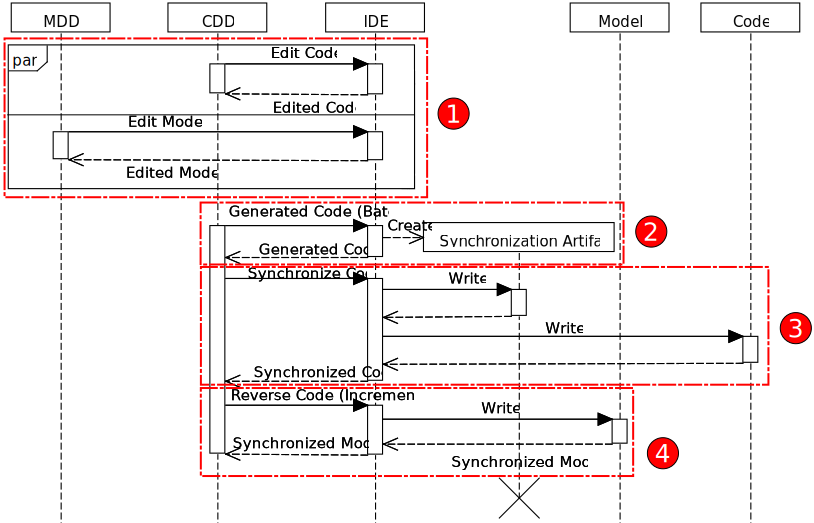
\includegraphics[width = \columnwidth]{figures/scenario3_seq}
\caption{Synchronization process, in which the model and the code are concurrently edited with code as the synchronization artifact (CDD = Code-Driven Developer, MDD = Model-Driven Developer). The API calls for Model and Code are represented generically as "Read" and "Write".}
\label{fig:scenario3}
\end{figure}

\begin{description}
	\item[Step 1] Both the model and code may be edited concurrently.
	(To simplify Figure \ref{fig:scenario3}, we don't show the Read and Write interactions for this step.)
	After both artifacts have been edited concurrently, we need to synchronize them.	
	\item[Step 2] First we create a synchronization artifact from the edited model by generating code in batch mode.
	This synchronization artifact is code and it is an image of the edited model.	
	\item[Step 3] The synchronization artifact is synchronized with the edited code. Since the synchronization artifact
is code itself, this step is done with the \texttt{Synchronize Code} use-case of the IDE.
	\item[Step 4] Once synchronization artifact and edited code are synchronized, the former is reversed incrementally to update the edited model.
\end{description}

The second strategy, based on using model as the synchronization artifact,
is the opposite of the first strategy. In the second strategy, the synchronization artifact is
obtained by reversing the edited code in batch mode.
Afterwards the synchronization artifact is synchronized with the edited model.
Finally, we generate code incrementally from the synchronization artifact to update the edited code.

%Figure \ref{fig:strategy2} shows the synchronization strategy based on using model as the synchronization artifact.
%This strategy is the opposite of the strategy presented in Figure \ref{fig:strategy1}. Its steps are described as follows:
%
%\begin{center}
%\textbf{\textit{- Steps of synchronization strategy 2 -}}
%\end{center}
%\begin{description}
%	\item[Step 1] The synchronization artifact is obtained by reversing the edited code in batch mode.
%	\item[Step 2] Afterwards the synchronization artifact is synchronized with the edited model.
%	\item[Step 3] Finally, we generate code incrementally from the synchronization artifact to update the edited code.
%\end{description}
%
%\begin{figure}
%\centering
%\includegraphics[width=\columnwidth]{figures/strategy2}
%\caption{Synchronization strategy 2 using model as synchronization artifact}
%\label{fig:strategy2}
%\end{figure}

We propose two strategies based on the preferences of the developers.
They may even use both strategies, successively, as a kind of hybrid strategy.
This may be useful
when developers want to synchronize parts of the system using one strategy,
and other parts using the other strategy. %For example, they may choose
%to synchronize method bodies using strategy 1, where the synchronization artifact is code.
%Then strategy 2, in which the synchronization artifact is a model, is used to
%to synchronize architectural elements of the system.

%In the next section we propose an implementation
%of an IDE and the proposed synchronization processes.

  %\input{sections/formalize}
  %\section{Round-trip engineering of UML State Machine and code}
\label{sec:approach}
This section presents our RTE approach. At first, it sketches USM concepts supported by this study. The outline and the detail of the approach are presented afterward.
\subsection{Scope}
A USM describes the behavior of an active UML class which is called context class. A USM has a number of possible states and well-defined conditional transitions. A state is either an atomic state, a composite state that is composed of sub-states and has at most one active sub-state at a certain time, or a concurrent state which has several active sub-states at the same time. Only one of the inner states of the USM can be active at a time. Transitions between states can be triggered by external or internal events. An action can also be activated by the trigger while transitioning from one state to another state. A state can have associated actions such as \ti{entry/exit/doActivity} executed when the state is entered/exited or while it is active, respectively. A transition can be external, local, or internal.

A composite state can have one or several entry/exit points. An entry/exit point can have multiple incoming transitions and exactly one outgoing transition which has no triggering event and guard. The transition outgoing from an entry point of a composite state ends on either a sub-state or an entry point of one of the sub-states of the composite state. The transition outgoing from an exit point ends on either an exit point of the parent state or a state/an entry point in the same region. A concurrent state is entered by either an incoming transition ending on its border, or several incoming transitions outgoing from a \ti{fork} and ending on sub-states of the containing regions. 

%UML SM is widely used as a means to modeling the behavior of a component in complex, reactive systems. A SM has a number of possible states and well-defined conditional transitions between states. A state is either an atomic state, a hierarchical state that is composed of sub-states and has at most one active sub-state at a certain time, or a concurrent state which could have several active sub-states at the same time. Only one of the inner states of the SM can be active at a time. A state can have associated actions such as entry/exit/doActivity executed in the running of the SM. The active state of the machine can be changed to another state triggered by external or internal events. An action can also be activated by the trigger in transitioning from one state to another one.  

\subsection{Approach outline}
Our RTE approach is based on the double-dispatch pattern presented in \cite{spinke_object-oriented_2013} for mapping from USM to a set of classes with embedded code fragments, and traceability-mapping management in RTE. Fig. \ref{fig:outline} shows the outline of our RTE approach consisting of a forward and a backward/reverse (engineering) process. In the forward process, a USM is transformed into UML classes in an intermediate model. The use of the intermediate model facilitates the transformation from the USM to code and vice versa. Each class of the intermediate model contains attributes, operations and method bodies (block of text) associated with each implemented operation. The transformation utilizes several patterns which will be presented later. A tracing information table is created in the transformation to be used in the backward direction of the RTE. The intermediate model is then used as the input of a code generator to create source code. This generation step also puts a mapping from UML classes to object-oriented source code in a second table.

When the source code is modified, a syntactic analysis process belonging to the backward transformation checks whether the modified code conforms to the USM semantics (see Subsection \ref{subsec:verification} for the detail of the analysis). This transformation takes as input the tracing tables, the created intermediate model and the USM to update these models sequentially. While the forward process can generate code from hierarchical and concurrent USMs, the backward one only works for hierarchical machines excluding some pseudo-states which are \ti{history}, \ti{join}, \ti{fork}, \ti{choice} and \ti{junction}. These features are in future work.

\begin{figure}
\centering
\includegraphics[clip, trim=3.5cm 3.5cm 5.9cm 3.5cm, width=1\columnwidth]{figures/flowchart.pdf}
\caption{Outline of state machine and code RTE} 
\label{fig:outline}
\end{figure}

\subsection{From UML state machine to UML classes}
This section describes the forward process which transforms a USM into an intermediate UML model. %The latter consists of transforming USM elements (see \ref{subsec:states}, \ref{subsec:events}, \ref{subsec:transitions}) into the intermediate model, storing tracing information (see \ref{subsec:trace}) and code generation (see \ref{subsec:codegen}) from the intermediate model.

\subsubsection{Transformation of states}
\label{subsec:states}
This sub-section describes the transformation of states to the intermediate model. 
%This paper considers a component as a UML class called context class. 
Each state of the USM is transformed into a UML class. Each UML class representing an atomic state inherits from a base state class. The latter defines a reference to the context class, a process event operation for each event in the USM and other operations as the double-dispatch (DD) approach in \cite{spinke_object-oriented_2013}. A state class \ti{s} also has an attribute referring to the state class associated with the composite state containing \ti{s}. A composite state class has an attribute pointing to a state instance indicating the active sub-state of the composite state and a \ti{dispatchEvent} operation (see \ref{subsec:codegen}) dispatching incoming events to the appropriate active state. A composite and a concurrent state class inherit from a base composite and base concurrent state class, respectively, which also inherit from the base state class. 
 %An example of this transformation in shown in Fig. \ref{fig:hierarchical-class}. The \ti{ParentState} and \ti{SubState} are vertexes of the SM describing the \ti{Client} component, for instance. The \ti{State} and \ti{CompositeState} classes are library classes. The \ti{ParentState} inherits from the \ti{CompositeState} class since it is a hierarchical state.

\begin{comment}
\begin{figure}
\centering
\includegraphics[clip, trim=6.5cm 21.3cm 5.5cm 2.4cm, width=0.5\textwidth]{figures/compositepattern}
\caption{Transformation from hierarchical state to class diagram} 
\label{fig:hierarchical-class}
\end{figure}
\end{comment}


\subsubsection{Transformation of events}
\label{subsec:events}
%DD has no means to convey data of events in the SM and considers every event as the same. In our approach, 
Each event is transformed into a UML class. Three different event class types corresponding to the UML event types \ti{CallEvent}, \ti{SignalEvent} and \ti{TimeEvent} are differentiated. An event class associated with a \ti{CallEvent} inherits from a base event class and contains the parameters in form of attributes typed by the same types as those of the operation associated with the \ti{CallEvent}. The operation must be a member of the context class (a component as described above). For example, a call event \ti{CallEventSend} associated with an operation named \ti{Send}, which has two input parameters typed by \ti{Integer}, is transformed into a class \ti{CallEventSend} having two attributes typed by \ti{Integer}. When a component receives an event, the event object is stored in an event queue.

A signal event enters the component through a port typed by the signal. The implementation view of this scenario depends on the mapping of component-based to object-oriented concepts. In the following, we choose the mapping done in Papyrus Designer \cite{_papyrus/designer/code-generation_????}. In this mapping, the signal is transferred to the context class by an operation provided by the class at the associated port. Therefore, the transfer of a signal event becomes similar to that of \ti{CallEvent}. For example, a signal event containing a data \ti{SignalData} arrives at a port \ti{p} of a component \ti{C}. The transformation derives an interface \ti{SignalDataInterface} existing as the provided interface of \ti{p}. \ti{SignalDataInterface} has only one operation \ti{pushSignalData} whose body will be generated to push the event to the event queue of the component. Therefore, the processing of a \ti{SignalEvent} is the same as that of a \ti{CallEvent}. In the following sections, the paper only considers \ti{CallEvent} and \ti{TimeEvent}.

A \ti{TimeEvent} is considered as an internal event. The source state class of a transition triggered by a \ti{TimeEvent} executes a thread to check the expiration of the event duration as in \cite{Niaz2004} and puts the time event in the event queue of the context class. 

\subsubsection{Transformation of transitions and actions}
\label{subsec:transitions}
%In this paper, actions, transition guards and effects in the SM are considered as an operation associated with a block of code describing the actions behavior. 
Each action is transformed into an operation in the transformed context class. \ti{Entry/Exit/doActivity} actions have no parameters while transition actions and guards accept the triggering event object. % have access to the event data. 
\ti{doActivity} is implicitly called in the \ti{State} class and executed in a thread which is interrupted when the state changes. A transition is transformed into an operation taking as input the source state object and the event object similarly to DD. Transitions transformed from triggerless transition which has no triggering events accept only the source state object as a parameter.

Four ways of entering a composite state are differentiated. Three of these including a transition ending (1) on the border, (2) on a sub-state or (3) on a history state of a composite state are detailed in \cite{spinke_object-oriented_2013}. In the last one, a transition \ti{$t_{ex}$} ends (4) on an entry point of a composite state. Semantically, (4) is similar to (2) since both have the same sequential operations: executing the entry action of the composite state, execute the effect of the outgoing transition of the entry point \ti{$t_{in}$} in (4) or the transition \ti{$t_{default}$} from an initial pseudo state to the sub-state in (2). The transition \ti{$t_{in}$} is not allowed to have a guard or a trigger event similarly to the semantics of \ti{$t_{default}$}. 

Exiting a composite state is executed through exit points inversely to entry points. %In our implementation presented in Section \ref{sec:implementation} entry points and exit points are supported in both directions of the RTTRIP. 

\subsubsection{Storage of tracing information}
\label{subsec:trace}
The tracing information generated in the transformation is contained in a table. Mappings from USM concepts to UML classes are mainly one-to-one except for attributes referring composite state or sub-state. The table therefore only keeps identifiers as qualified names and types of elements in the USM model and the associated elements in the UML class model. A part of tracing table for the USM example in Fig. \ref{fig:statemachuine} is shown in Table \ref{table:trace} in which \ti{sPrefix} and \ti{tPrefix} are \ti{Root::Client::StateMachine::TopRegion} and \ti{Root::Client::PerClass\_Client}, respectively.

In Fig. \ref{fig:statemachuine}, the USM is contained in, for instance, a \ti{Client} component, \ti{Root} is the name of the source model. States of the USM are contained in a region \ti{TopRegion}. In the intermediate model, a package named \ti{PerClass\_Client} is created to contain all of transformed classes including ones associated with events and states. This package eases the maintenance of source code as well as the backward transformation of the RTE. The transition \ti{fromStoppedToOperating} is transformed into an operation transition inside the USM class which contains \ti{Stopped}. \ti{Initialize}, \ti{Enable}, \ti{Prepare}, and \ti{Disable} are transformed into operations in the context class \ti{Client}. It is worth noting that there can be several transitions outgoing from a state. Therefore, more than one transition in USM can be mapped to the same qualified name in the tracing table. In order to differentiate different transitions in the intermediate model, the qualified name of a transition operation in the intermediate model is combined with the source state and the triggering event. From this tracing table, it is easy to look back the original USM elements from the elements in the intermediate model in the backward direction. %This transformation can be implemented as an in-place transformation but it would surprise users. Furthermore, the intermediate model should be used only as a bridge to the code and hidden to users. 

\begin{figure}
\centering
\includegraphics[clip, trim=2.5cm 22.5cm 10.8cm 2.5cm, width=0.8\columnwidth]{figures/statemachine}
\caption{An example of USM for tracing table} 
\label{fig:statemachuine}
\end{figure}

\begin{comment}
\begin{table*}[]
\centering
\caption{Tracing table of state machine and class intermediate model}
\label{table:trace}
\begin{tabular}{|l|l|}
\hline
\rowcolor{Gray}
UML state machine concepts                                                 & UML class concepts                                     \\ \hline
Root::Client::StateMachine::TopRegion::Stopped (State)                     & Root::Client (Class)                                   \\ \hline
Root::Client::StateMachine (StateMachine)                                  & Root::Client::PerClass\_Client::StateMachine (Class)   \\ \hline
Root::Client::StateMachine::TopRegion::Stopped (State)                     & Root::Client::PerClass\_Client::Stopped (Class)        \\ \hline
Root::Client::StateMachine::TopRegion::Operating (State)                   & Root::Client::PerClass\_Client::Operating (Class)      \\ \hline
Root::Client::StateMachine::TopRegion::On (CallEvent)                      & Root::Client::PerClass\_Client::On (Class)             \\ \hline
Root::Client::StateMachine::TopRegion::Initialize(OpaqueBehavior)          & Root::Client::PerClass\_Client::Initialize (Operation) \\ \hline
Root::Client::StateMachine::TopRegion::Enable (OpaqueBehavior)             & Root::Client::PerClass\_Client::Enable (Operation)     \\ \hline
\end{tabular}
\end{table*}


\begin{table}[]
\centering
\caption{Tracing table of state machine and class intermediate model}
\label{table:trace}
\begin{tabular}{|l|l|}
\hline
\rowcolor{Gray}
UML state machine concepts                                                 & UML class concepts                                     \\ \hline
sPrefix::Client (Class)                     & Root::Client (Class)                                   \\ \hline
Root::Client::StateMachine  (StateMachine)                                  & tPrefix::StateMachine (Class)   \\ \hline
sPrefix::Stopped (State)                     & tPrefix::Stopped (Class)        \\ \hline
sPrefix::Operating (State)                   & tPrefix::Operating (Class)      \\ \hline
sPrefix::On (CallEvent)                      & tPrefix::On (Class)             \\ \hline
sPrefix::fromStoppedToOperating (Transition) & tPrefix::StateMachine::transition (Operation) \\ \hline
sPrefix::Initialize(OpaqueBehavior)          & tPrefix::Initialize (Operation) \\ \hline
sPrefix::Enable (OpaqueBehavior)             & tPrefix::Enable (Operation)     \\ \hline
\end{tabular}
\end{table}
\end{comment}
\subsubsection{Code generation}
\label{subsec:codegen}

The intermediate model is then used as input of a template-based object-oriented code generator. Mappings from UML classes to object-oriented are trivial one-1-one. Listing \ref{lst:code-segment} shows a code segment generated from the USM in Fig. \ref{fig:statemachuine}. The \ti{dispatchEvent} method implemented in the base composite state class delegates the incoming event processing to its active sub-state. If the event is not accepted by the active sub-state, the composite state processes it. \ti{OnEntryAction} and \ti{OnExitAction} overwrite abstract methods which are defined in the base state class and called by the entry and exit methods, respectively. \ti{Stopped} accepts an \ti{On} event by implementing a corresponding \ti{processEvent} method. The transition method from the \ti{Stopped} to the \ti{Operating} state checks the guard condition by calling an associated method in the context class, then executes the transition action, changes the active state and finally enters the target state by calling the entry operation. The machine enters the final state by setting the active state to null meaning that the behavior of the region containing the final state has completed. The generated code statements are identical to the USM semantics and it is easy to modify the behavior of the USM by code. %For example, if we would like to change the default state, we only need to modify the \ti{setInitDefaultState} method by assigning the attribute \ti{activeSubState} to the attribute \ti{operating} that represent an instance of the state \ti{Operating}.


\begin{algorithm}[tbp]
\caption{A segment of C++ generated code \label{lst:code-segment}}
\lstset{language=C++}
\begin{lstlisting}
class CompositeState: public State {
protected:
  State* activeSubState;
public:
bool dispatchEvent(Event* event) {
bool ret = false;
if (activeSubState != NULL) {
ret = activeSubState->dispatchEvent(event);}
return ret || event->processFrom(this);}}
StateMachine::StateMachine(Client* ctx){
  this->context = ctx;
  stopped = new Stopped(this, ctx);
  operating = new Operating(this, ctx);
  this->setIniDefaultState();
  this->activeSubState->entry();}
void StateMachine::setIniDefaultState(){
  this->context->Initialize();
  this->activeSubState = stopped;}
bool StateMachine::transition(
        Stopped* state, On* event) {
 if(this->context->guard(event)){
  this->activeSubState->exit();
  this->context->Enable(event);
  this->activeSubState = this->operating;
  this->activeSubState->entry();
  return true;}
return false;}
bool StateMachine::transition(
    Operating* state, Off* event) {
  this->activeSubState->exit();
  //no action defined
  this->activeSubState = NULL;
return true;}
class Stopped: public State {
private:
  StateMachine* ancestor;
public: 
virtual bool processEvent(On* event) {
  return ancestor->transition(this,event);}
}
\end{lstlisting}
\end{algorithm}


\subsection{Reverse engineering from code to USM}
This section describes the backward process. 

\subsubsection{Method Overall}
%The modifications made to the generated code need to be reversed back to the SM to make the artifacts consistent. 
The overall method for backward transformation is shown in Fig. \ref{fig:details}. The modified code is first analyzed by partly inspecting the code syntax and semantics to guarantee that it is reversible. There are cases in which not all code modifications can be reversed back to the USM. The analysis also produces an output (\ti{output2}) whose format is described later. If the intermediate model or the original USM is absent (the lower part of Fig. \ref{fig:details}), a new intermediate model and a new USM are created from the UML model. In the contrary, the previous code taken, for instance, from control versioning systems is also semantically analyzed to have its output (\ti{output1}) (the upper part of Fig. \ref{fig:details}). \ti{Output1} and \ti{Output2} are then compared with each other to detect actual semantic changes which are about to be propagated to the original model. 

\begin{figure}
\centering
\includegraphics[clip, trim=0.9cm 5.8cm 15.1cm 6.3cm, width=0.8\columnwidth]{figures/details2.pdf}
\caption{Overall method for reversing code to state machine} 
\label{fig:details}
\end{figure}

\subsubsection{Semantic Analysis}
\label{subsec:verification}
The output of the semantic analysis contains a list of event names, a list of state names, a list of transitions in which each has a source state, a target state, a guard function, an action function and an event represented in so called abstract syntax tree (AST) transition [15]. 
For example, Fig. \ref{fig:transitions} presents the EMF \cite{gronback_eclipse_} representation of transitions in a \tb{C++} AST in which \ti{IStructure} and \ti{IFunctionDeclaration} represent a structure and a function in \tb{C++}, respectively. 
Each state name is also associated with an ancestor state, an entry action, an exit action, a default sub-state and a final state. 
The output is taken by analyzing the AST. 
The analysis process consists of recognizing different patterns. 
The pattern list is as followings:

\noindent
\tb{State}: A state class inherits from the base state class or the composite base state class. 
For each state class, there must exist exactly one attribute typed by the state class inside another state class. 
The latter becomes the ancestor of the state class.

\noindent
\tb{Composite state}: A composite state class (CSC) inherits from the base composite state. 
For each sub-state the CSC has an attribute typed by the associated sub-state class. 
The CSC also implements a method named \ti{setInitDefaultState} to set its default state. 
The CSC has a constructor is used for initializing all of its sub-state attributes at initializing time.

\noindent
\tb{Entry action}: If a state has an entry action, its associated state class implements \ti{onEntryAction} that calls the corresponding action method implemented in the context class. 

\noindent
\tb{Activity/Exit action}: Similar to the entry action pattern but implements \ti{onExitAction}/\ti{onActivity}, respectively. 
According the USM semantics, if an atomic state has outgoing \ti{triggerless} transitions, \ti{onEntryAction} appeals the \ti{triggerless} transition method of the ancestor state class following the  \ti{onActivity} call. For composite states, the \ti{triggerless} transition method is called after the its active sub-state is a final state (NULL from implementation perspective) and its activity completes. Note that thread-based parallelism of \ti{doActivity} is implicitly implemented (not presented here) and called by the base state classes which are generated by the generator. Therefore, for each state class added to the code side, developers only need to overwrite the appropriate action methods from the base state classes. This facilitates the analysis and extraction of state actions/events to reconstruct USMs from code within the reverse engineering task.

%\tb{Exit action}: Similar to the entry action pattern but implements \ti{onExitAction}.

\noindent
\tb{Event processing}: If a state has an outgoing transition triggered by an event, the class associated with the state implements the \ti{processEvent} method having only one parameter typed by the event class transformed from the event. 
The body calls the corresponding transition method of the ancestor class.

\noindent
\tb{CallEvent} class: A call event class inherits from the base event class. 
The call event class contains attributes typed by the parameter types of the operation associated with the call event. 
This pattern is detected if the types of attributes of the event class match with the types of parameters of one of the methods in the context class. 
There is therefore an ambiguity for an event class to choose an associated operation if more than one operation detected matches the event class. 
Hence, this pattern poses a restriction that operations associated with events must either have different parameter types or different number of parameters. 
To overcome this issues, a naming convention used for \ti{CallEvent} classes is used. 
The event class name is prefixed with the associated operation name. 
If the event class name does not follow the naming convention, the reverse is refused. 
Another possible solution targeting this ambiguity is to have a user interaction in case of having more than one operation matching with the event. 
Having an interaction allows the pattern detection get rid of ambiguity and therefore provides appropriate USM models. 
A signal event is treated as a \ti{CallEvent} as previously described.

\noindent
\tb{Time event}: A transition is triggered by a \ti{TimeEvent} if the state class associated with its source state implements the timed interface. 
The duration of the time event is detected in the transition method whose name is formulated as \ti{"transition" + duration}. 

\noindent
\tb{Transition}: Transition methods are implemented in the ancestor class, which is the class associated with the composite state owning the source state of the transition. 
Two types of transition methods correspond to trigger and \ti{triggerless} transitions. 
Both \ti{parameterize} its source state class. 
The trigger transition method is associated with the event triggering the transition. 
The body of external and internal transition methods contains ordered statements including exiting the source state, executing transition action (effect), changing the active state to the target or null if the target is the final state, and entering the changed active state by calling entry. 
The body can have an if statement to check the guard of the transition. 
The transition action and the guard are optional. 
Several if/else statements can appear in a \ti{triggerless} transition method body. 
The body of local transition methods only checks its guard and executes the transition effect.

\noindent
\tb{Transition action/guard}: Transition actions and guards are implemented in the context class.

\begin{algorithm}[]
  \caption{Semantic Analysis
    \label{alg:semantic-vefrification}}
  \begin{algorithmic}[1]
    \Require{AST of code and a list of state classes stateList}
	\Ensure{Output of semantic analysis}
    %\Statex
    	\For {$s$ in $stateList$}
        	\For {$a$ in attribute list of $s$}
        		\If {$a$ and $s$ match child parent pattern}
        			\State put a and s into a state-to-ancestor map;
        		\EndIf
        	\EndFor
        	\For {$o$ in method list of $s$}
        		\If {$o$ is $onEntryAction$ || $o$ is $onExitAction$}		
        			\State $analyzeEntryExit(o)$; 	
        		\ElsIf {$o$ is $processEvent$} 
        			\State $analyzeProcessEvent(o)$;
        		\ElsIf {$o$ is $setInitDefaultState$ \& $s$ is composite}
        			\State $analyzeInitDefaultState(s)$;
        		\ElsIf {$o$ is timeout \& $s$ is a timedstate}
        			\State $analyzeTimeoutMethod(o)$;
        			\State $analyzeProcessEvent(s,o)$;
        		\EndIf	
        	\EndFor
    	\EndFor
  \end{algorithmic}
\end{algorithm}

Algorithm \ref{alg:semantic-vefrification} shows the algorithm used for analyzing code semantics. Due to space limitation, \ti{analyzeEntryExit}, \ti{analyzeProcessEvent}, \ti{analyzeInitDefaultState}, \ti{analyzeTimeoutMethod} and \ti{analyzeProcessEvent} are not presented but they basically follow the pattern description as above. In the first step of the analysis process, for each state class, it looks for an attribute typed by the state class, the class containing the attribute then becomes the ancestor class of the state class. The third steps checks whether the state class has an entry or exit action by looking for the implementation of the \ti{onEntryAction} or \ti{onExitAction}, respectively, in the state class to recognize the \ti{Entry/Exit} action pattern. Consequently, event processing, initial default state of composite state and time event patterns are detected following the description as above.  Fig. \ref{fig:partition} shows the partitioning used for matching code segments to USM elements. Each partition consists of a code segment and the corresponding model element which are mapped in the backward direction. For instance, the \ti{Stopped} class in code is detected as a representation since it inherits from the base class \ti{State}.  
 
\begin{comment}
\begin{figure}
\centering
\includegraphics[clip, trim=1cm 4.8cm 0.1cm 0.8cm, width=0.75\textwidth]{figures/backwardmapping.pdf}
\caption{USM element-code segment mapping partition} 
\label{fig:partition}
\end{figure}
\end{comment}

\begin{figure*}
\centering
\includegraphics[clip, trim=1.8cm 5.55cm 2.1cm 3.8cm, width=1\columnwidth]{figures/bkwmapping.pdf}
\caption{USM element-code segment mapping partition} 
\label{fig:partition}
\end{figure*}

\begin{figure}
\centering
\includegraphics[clip, trim=0cm 0.6cm 0.0cm 0.6cm, width=\columnwidth]{figures/asttransition}
\caption{Transitions output from the analysis} 
\label{fig:transitions}
\end{figure}

\subsubsection{Construction of USM from analysis output}
If an intermediate model is not present, a new intermediate model and a new USM are created by a reverse engineering and transformation from the output of the analysis process. The construction is straightforward. At first, states are created. Secondly, UML transitions are built from the AST transition list. Lastly, action/guard/triggering event of a UML transition is created if the associated AST transition has these.

\subsubsection{Updating the original USM from modified code}
In contrast to the previous sub-section, if an intermediate model is existing, lists of states and transitions are retrieved from the intermediate model. 
%The output of the verification process and that of the intermediate model transformation are compared to each other to detect semantics changes of the modified code. 
The algorithm for detecting state and transition changes is not presented here due to space limitation. Basically, the algorithm takes as input lists of state names, transitions, ancestor maps, which link a state name to its parent state name, extracted from the intermediate model and the modified code, respectively. The algorithm results in lists of state names, transitions to be added/deleted/updated/moved. It first examines the list of state names extracted from the modified code $Lc$ to find which state to be added. A state is considered as a to-be-updated state if its name exists in both of the two lists of state names and its ancestor names in both of the ancestor maps are identical. If the latter condition is not satisfied, the state is considered as being moved to another composite state. Remaining states (not added/updated/moved) in the state list extracted from the intermediate model are added to the to-be-deleted state list. The transition and event change detection is similar to that of states but, due to the space limitation, it is not detailed. For transition change detection, instead of checking by name, the source and target state names of transitions and the associated event name in transitions are used.
%It first examines the list of state names extracted from the modified code $Lc$ for states that are not existing in the list of state names of the intermediate model $Li$ to be added to the added state list. If a state $c$ in $Lc$ is present in $Li$, $c$ is either added to the updated list if the ancestor states associated with $c$ in the intermediate model and the modified code are the same, or $c$ is considered as being moved to another ancestor state. Other states in $Li$ are added to the deleted state list. The transition and event change detection is similar to that of states but, due to the space limitation, it is not detailed. For transition change detection, instead of checking by name, the source and target state names of transitions and the associated event name in $Tc$ and $Ti$ are used. 

The changes detected by the algorithm are then used in a change propagation step which updates the original USM. Events, states and transitions are sequentially processed in order. The processing of elements to be deleted results in deleting corresponding elements in the USM. As previously described, the mapping information for elements in code and the intermediate model is also stored in a table. Each to-be-deleted element in code is associated with an element in the intermediate model. Therefore, it is trivial to retrieve the model element in the intermediate model associated with the to-be-deleted element.

The found model element in turn helps identify the associated element in the USM by using the mapping table between the USM and the class model. For each deleted event in code, the associated event class in the class model and the event in the USM are deleted. Deleted states and transitions are similarly propagated. A deletion of a transition includes deleting its guard, triggers and transaction action. 

\begin{comment}
\begin{algorithm}[H]
  \caption{Change detection
    \label{alg:change-detect}}
  \begin{algorithmic}[1]
    \Require{$Li$, $Lc$, $Ti$, $Tc$, $mapI$, $mapC$ are lists of state names, transitions, ancestor map extracted from intermediate model and modified code, respectively}
	\Ensure{$adS$, $delS$, $uptS$, $movS$ are lists of added, deleted, updated and moved states respectively. $adT$, $delT$, $uptT$ are lists of added, deleted and updated transitions}
    %\Statex
    	\For {$c$ in $Lc$}
        	\If {!$Li$.contains($c$)} 
				\State adS.put(c);
        	\Else
				\If {$mapC$.get($c$) = $mapI$.get($c$)}
	    			\State uptS.put(c);
				\Else 
	    			\State $movS$.put($c$, $mapI$.get($c$), $mapC$.get($c$))	
                \EndIf
                	\State $Li$.remove($c$);
        	\EndIf
    	\EndFor
    	\For {$i$ in $Li$} 
        	\State $delS$.put($i$)
    	\EndFor
    	\For {$c$ in $Tc$}
        	\State $found$ = NULL
        	\For {$i$ in $Ti$}
				\If {$c$.source=$i$.source \& $c$.target=$i$.target \& $c$.event = $i$.event}
	    			\State $found$ = $i$;
              	\EndIf
             \EndFor 	
        	\If {$found$ != NULL} 
				\State $uptT$.put($c$);
				\State $Ti$.remove($found$);
        	\Else
				\State $adT$.put($c$);
        	\EndIf
    	\EndFor
    	\For {$t$ in $Ti$}
        	\State $delT$.put($t$);
    	\EndFor
  \end{algorithmic}
\end{algorithm} 
\end{comment}

\begin{comment}
\begin{algorithm}[H]
  \caption{Change detection
    \label{alg:change-detect}}
  \begin{algorithmic}[1]
    \Require{$Li$, $Lc$, $Ti$, $Tc$, $mapI$, $mapC$ are lists of state names, transitions, ancestor map extracted from intermediate model and modified code, respectively}
	\Ensure{$adS$, $delS$, $uptS$, $movS$ are lists of added, deleted, updated and moved states respectively. $adT$, $delT$, $uptT$ are lists of added, deleted and updated transitions}
    %\Statex
    	\For {$c$ in $Lc$}
        	\If {!$Li$.contains($c$)} 
				\State adS.put(c);
        	\Else
				\If {$mapC$.get($c$) = $mapI$.get($c$)}
	    			\State uptS.put(c);
				\Else 
	    			\State $movS$.put($c$, $mapI$.get($c$), $mapC$.get($c$))	
                \EndIf
                	\State $Li$.remove($c$);
        	\EndIf
    	\EndFor
    	\For {$i$ in $Li$} 
        	\State $delS$.put($i$)
    	\EndFor
    	\State $detect transition changes$;
  \end{algorithmic}
\end{algorithm} 
\end{comment}

For each event class added to code, a UML class is added to the intermediate model and a UML event to the USM. For each added state class, its ancestor state is retrieved through the mapping tables, a new state is then created as a sub-state of the ancestor state. Entry and exit actions are added to the new state afterward. A moved state is handled by looking for the associated state, the old and new ancestor state in the USM, and moving the associated state to the new ancestor state. Each added transition is propagated by creating a new transition in the USM and retrieving source and target states from the mapping tables. An update is executed by looking in the mapping tables for elements in the USM associated with elements updated in code. %It is worth noting that this algorithm detects a renaming of an event or state as a deletion followed by an addition. 


  
For example, assuming that we need to adjust the USM example shown in Fig. \ref{fig:statemachuine} by adding a guard to the transition from \ti{Operating} to the final state. The adjustment can be done by either modifying the USM model or the generated code. In case of modifying code, the associated transition function in Listing \ref{lst:code-segment} is edited by inserting an \ti{if} statement which calls the guard method implemented in the context class. The change detection algorithm adds the transition function into the updated list since it finds that the source state, the target state and the event name of the transition is not changed. By using mapping information in the mapping table, the original transition in the USM is retrieved. The guard of the original transition is also created. 	






   \section{A complete code generation solution for UML State Machine}
\label{sec:codegen}
This section describes a complete generation solution for UML State Machine, especially when considering the concurrency aspect. It first reminds background definitions in a formal way and some assumptions on output generated code. 
Subsection \ref{sec:thread} continues with the concurrency design for generated code based on multi-thread. 
Overview of a code generation approach based on the design is then discussed. %before a synchronization approach is introduced.

\input{sections/formalize} 

\subsection{Thread-based Concurrency for UML State Machine}
\label{sec:thread}
This Subsection describes our design for generated code. 
The design is based on an example-based analysis, which is not presented here due to space limitation.

%\subsubsection{Thread-based concurrency analysis} 

%While concurrency is an important aspect defined by the UML State machine specification, especially hierarchical and concurrent state machines with \ti{doActivity}s for states, most of existing approaches do not take into account. This is non-trivial since concurrency is dynamic in UML state machine and the number of threads used for concurrency is non-deterministic.



Let us give an analysis on the state machine example in Fig. \ref{fig:example}. Assuming that \ti{Idle} is the current active state and a \ti{verifyPIN} event is coming. 
The \ti{doActivity} behavior of \ti{Idle} \ti{doActivity(Idle)} (if has) is terminated, \ti{exit(Idle)} and the \ti{effect(t2)} (\ti{T2Effect}) are executed sequentially. 
These actions are run in a state machine main thread which reads incoming events from a "first in, first out" (FIFO) priority queue. 
Fig. \ref{fig:threading1} shows the activity diagram representing the concurrency processing \ti{verifyPIN}, in which each partition represents a thread. 
\ti{effect(t3)} and \ti{effect(t3)} are run concurrently in two threads \ti{T3Run} and \ti{T4Run}, respectively, since the transitions owning these effects outgo from a fork pseudo state. 
The entry action \ti{entry(Verifying)} is executed following the termination of the two threads. 

UML says that \ti{doActivity(Verifying)}, \ti{entry(VerifyingCard)} and \ti{entry(VerifyingPIN)} should be concurrently executed upon the completion of \ti{entry(Verifying)}, which is represented by a fork node, in which a \ti{Start} signal is sent to \ti{VerifyingDoRun} in order for commencing \ti{doActivity(Verifying)}. 
The executions of the \ti{doActivity}s of the states \ti{VerifyingCard} and \ti{VerifyingPIN} are also concurrent. 
Also, upon the completion of \ti{entry(VerifyingCard)} and \ti{entry(VerifyingPIN)}, the main thread completes the processing of the \ti{verifyPIN} event, reads next events from the queue or waits for next event occurrences.

\begin{figure}
	\centering
	\includegraphics[clip, trim=1.0cm 1.6cm 1.6cm 1cm, width=1.03\columnwidth]{figures/ThreadingExample.pdf}
	\caption{Concurrency of the ATM when receiving the \ti{verifyingPIN} event} 
	\label{fig:threading1}
\end{figure}

If no event is coming, and \ti{doActivity(VerifyingCard)} and \ti{doActivity(VerifyingPIN)} are long actions (e.g. forever loops inside), the state machine remains its active configuration and three concurrent actions including \ti{wait for events}, \ti{doActivity(VerifyingCard)}, and \ti{doActivity(VerifyingPIN)} are permanently run.

The termination time of \ti{doActivity(VerifyingCard)} and \ti{doActivity(VerifyingPIN)} is non-deterministic. 
However, a completion event is generated and pushed to the event queue whenever one of the two completes. 

\begin{comment}
For illustration, assuming that \ti{doActivity(VerifyingCard)} terminates before \ti{doActivity(VerifyingPIN)}. 
As in Fig. \ref{fig:threading2}, the Main thread checks the \ti{CompletionEvent}. \ti{exit(VerifyingCard)} and \ti{effect(t5)} are then executed sequentially. If \ti{cardValid} is computed as true as the result of \ti{doActivity(VerifyingCard)} and \ti{exit(VerifyingCard)}, the Main thread simply executes \ti{effect(t6)} and \ti{entry(CardValid)} before waiting for other events.

In contrast, Main sends a signal to stop \ti{doActivity(VerifyingPIN)} and \ti{doActivity(Verifying)}, executes exit, transition and entry actions in an appropriate order (see Fig. \ref{fig:threading2}) and waits for other events.

\begin{figure}
\centering
\includegraphics[clip, trim=1.5cm 1.6cm 1.6cm 1.2cm, width=1.03\columnwidth]{figures/ThreadingExample2.pdf}
\caption{Concurrency of the ATM when \ti{doActivity} of \ti{VerifyingCard} completes before that of \ti{VerifyingPIN}}
\label{fig:threading2}
\end{figure}
\end{comment}

We see that the number of concurrent actions is not constant but changes timely. 
Each action can either deterministically or non-deterministically terminate. 
In this sense, deterministic actions (DAs) prevent the Main thread from going to the waiting-for-event point. 
In other words, pending events in the queue are only read and processed once all deterministic actions complete. Therefore, we re-define the run-to-completion paradigm of UML state machine as following:
 
\begin{definition}
	Run-to-completion means that, in the absence of exceptions or asynchronous destruction of the context	class object or the state machine execution, a pending Event occurrence is dispatched only after the completion of all deterministic actions commenced by the processing of the current event. 
	At this point, a stable state configuration has been reached
\end{definition}

%In the example, some of DAs are as followings: \ti{effect(t2)}, \ti{effect(t4)}, \ti{entry(Verifying)}, \ti{entry(VerifyingCard)}, and non-deterministic actions (NDAs) as followings: \ti{doActivity(Verifying)}, \ti{doActivity(VerifyingCard)} and \ti{doActivity(VerifyingPIN)}.




\subsubsection{Thread-based design of generated code}
The concurrency of concurrent UML State Machines is based on multi-thread, in which there are permanent and spontaneous threads. 
While permanent threads (PTs) are created once and live as long as the state machine is alive, spontaneous threads (STs) are spawned in active for a while. 
%The method associated with a permanent thread is a non-deterministic action, which is run in parallel with the main thread. The latter reads and dispatch events from the event queue. 
Each PT is initialized at the state machine initialization. 
%The number of threads associated with NDAs is therefore equal to that of the NDAs.
The design of threads is based on the thread pool pattern, which initializes all threads at once, and the paradigm "wait-execute-wait". 
In the latter, a thread \tb{waits} for a signal to \tb{execute} its associated method and goes back to the \tb{wait} point if it receives a stop signal or its associated method completes. 
Each PT is associated with one of the following actions:
\begin{itemize}
	\item \ti{doActivity} of each state if has. %The number of \ti{doActivity} $n_{do} = \#\{s \in V|\exists doActivity(s)\}$
	
	\item Sleep function associated with a \ti{TimeEvent} which counts ticks and emits a \ti{TimeEvent} once completes.%: $n_{te} = \#\{e \in E|\ti{e is a time event}\}$.
	
	\item Change detect function associated with a \ti{ChangeEvent} which observes a variable or a boolean expression and pushes an event to the queue if changes happen.%: $n_{che} = \#\{e \in E|\ti{e is a change event}\}$.
	
	\item State machine main thread,which reads events from the event queue, and sends start and stop signals to these initial threads.
\end{itemize} 

%Therefore, The number of initial threads is $n_{threads} = n_{do} + n_{te} + n_{che}$ plus a main thread, which reads events from the event queue, and sends start and stop signals to these initial threads. 

Now we consider STs which are spawned by a parent thread, joined until and destroyed once the associated methods complete. 

\begin{comment}
The followings describe different types of DAs:

\begin{itemize}
	\item Actions executed when entering/exiting an orthogonal region, which can be: execute a chain of transition effects contained by the region before entering a stable sub-state or exiting the region completely.%: $n_{region threads} = \#\{r \in \mathcal{R}|ctner(r).kind=conc\}$
	
	\item Effects of transitions outgoing from a $fork$ and those incomings to a $join$.%: \\
	%$\mathcal{J} = \{v \in V|v.kind=join\}$ \\
	%$\mathcal{F} = \{v \in V|v.kind=fork\}$ \\
	%$$n_{FJ\_threads} = \sum_{v \in \mathcal{F}} {\#T_{outs}(v)} + \sum_{v \in \mathcal{J}} {\#T_{ins}(v)}$$.
\end{itemize}
\end{comment}

The STs follow a paradigm in which if a thread $parent$ spawns a set of threads $children$, $parent$ must wait until $children$ complete their associate methods. These threads are spawned in one of the following cases:

\begin{itemize}
	\item A thread is created for each effect of transitions' outgoing from a \ti{fork} or incoming to a \ti{join}.
	
	\item Entering a concurrent state $s$, after the execution of $entry(s)$, a thread is also created for each orthogonal region. 
	
	\item Exiting a concurrent state $s$, before the execution of $exit(s)$, a thread is also created for each region to exit the corresponding active sub-state.
	
	%\item An event is processed by active states, in which a thread per orthogonal region. 
\end{itemize}

\subsubsection{Deadlock avoidance}
Each PT is associated with a mutex for synchronization communication in the multi-thread-based generated code. 
The mutex must be locked before the method associated with the thread is executed. 
The mutex associated with the main thread preserves the run-to-completion semantics since some event such as \ti{CallEvent} can be processed synchronously and some asynchronously. Each event processing must lock the main mutex before executing the actual processing. 
%Deadlock is one of the main issues in designing multi-thread applications, in which two competing actions wait for the other to finish. In our case, 


\begin{comment}
\begin{tabular}{p{4.0cm}|p{4.0cm}}
Example code generated for doActivity  &  Option  2\\
\begin{lstlisting}[language=C++]
void doActivity(int stateId) {
  isStarts[stateId] = false;
  while(true) {
    mutex[stateId].lock();
    while(!isStarts[stateId]) {
      mutex[stateId].wait();
    }
    states[stateId].doActivity();
    isStarts[stateId] = false;
    mutex[stateId].unlock();
    if (!isStops[stateId]) {
      if (stateId == IDLE_ID || stateId == DISPENSEMONEY_ID ...) {
	    pushCompletionEvent(stateId);
	  }
    }
  }
}
	\end{lstlisting}&
	\begin{lstlisting}
	#include <stdio.h>
	
	int main()
	{
	printf("Hello world\n");
	}
	\end{lstlisting}
\end{tabular} 
\end{comment}


%\subsection{Transformation pattern}
%todo: describe the pattern

%Transformation from State machine to fUML (classes, attributes, methods)
%\lipsum[1]

\subsection{Assumption}
%todo: give some assumptions on code generation such as functions to create methods, attriutes, classes
Assuming that we want to generate from the state machine to an object oriented programming language $ActLang$, which is C++-like and supports multi-threading as following functions and resource control as mutexes.
\begin{itemize}
	%\item $genClass(n, generals, itfs)$ creates a class with its name, parent class set, and implemented interfaces as \ti{n}, \ti{generals}, and \ti{itfs}.
	
	%\item $genMtd(n, c, type, params)$ creates a method $m$ with its name as $n$ inside the class $c$, its return type as $type$, and $params$ as its parameter set.
	
	%\item $genAttr(n, c, type, multiplicity)$ creates an attribute named $n$ in the class $c$ and typed by $type$. The create attribute is an array if $multiplicity > 1$, otherwise a simple attribute.
	
	%\item $genEnum(n)$ and $genEnumLit(enum, n)$ create an enumeration and its enumeration literal, respectively.
	
	%\item $genBody(m, body)$ adds a body to a method. The body is a string which contains a list of statements.
	
	%\item $createParalle(t, seg)$ generates a mechanism which allows the segment code $seg$ run in a thread $t$. Similarly, $genWait(t), genJoin(t)$.
	
	\item A mutex has three methods $lock$, $unlock$, and $wait$, which automatically unlocks the mutex and waits until it receives a signal.  
	
	%\item $synchronize(seg)$ generates a mechanism which allows the segment code $seg$ run safely (can be either based on \ti{POSIX pthread} or \ti{Java synchronize} mechanism).
	
	%\item $toString(stts)$ is used to convert a list of statements $stts$ into a readable string which can be add to a method as its body.
	
	%\item Concatenation of two strings $str1$ and $str2$ is concisely described as $str1 + str2$.
	
	%\item \ti{WHILE}, \ti{FOR} \ti{IF}, \ti{ELSE} are symbols representing while and for loops, if and else statements.
	
	\item \ti{FORK(func)} creates a thread (lightweight process) associated with the function/method \ti{func} and \ti{JOIN(theThread)} waits until the method associated with the thread \ti{theThread} completes.
\end{itemize} 

\subsection{Code generation pattern}

\subsubsection{State transformation}
%Suppose that we want to generate a state machine $sm$ whose states are listed by $lstates$. 
A common state interface $IState$ is created. The interface contains three methods, namely, \ti{entry}, \ti{exit}, and \ti{doActivity} respectively corresponding to three state actions. To preserve the hierarchy of composite states, the interface also has two attributes called \ti{actives} and \ti{previousActives} referring to current and previous active sub-states in case of the presence of history states, and a list of deferred event identifiers.

Each UML state is transformed into an instance of the interface associated with a state ID (which is a child element of an enumeration) inside the active class $C$. 
During initialization, each instance delegates its methods to suitable implementation, e.g. function pointers in C++. 
%In other object-oriented languages such as Java, this is done with anonymous sub-classes of the interface. 
For example, Listing \ref{lst:IStateCpp} in Appendix shows the interface and its instances. 
%The actions of the states are named depending on the name of the states. In the following sections, we only consider \ti{ActLang} as a C++-like. The discussion of other object-oriented languages are much similar since these share the same concepts.

Each \ti{doActivity} is associated with a permanent thread and a mutex. The \ti{doActivity} thread is initialized, waits for a start signal, executes the \ti{doActivity} code, generates a completion if the state is atomic and still active, and goes back to the waiting point as the paradigm above. Listing \ref{lst:doActivity} in Appendix shows a code segment for \ti{doActivity} threads. 




\begin{comment}
\begin{lstlisting}[mathescape=true, caption=IState interface and annonymous sub-classes in Java, label=lst:IStateJava, frame=single, language=JAVA]
public interface IState {
  public IState[] pres; 
  public IState[] actives;
  public EventId defEvents;
  public void entry();
  public void exit();
  public void doActivity();
}
class C {
private IState states[NUM_STATES];
public C() {
  states[S0_ID] = new IState() {
    public void entry() {
      S0_entry();
    }
    ...
  }
}
public void S0_entry() {...}
}
\end{lstlisting}
\end{comment}

\begin{comment}
The procedure to generate the code for states is shown in Listing \ref{lst:procedure1}. It first creates the state interface $IState$ (in C++, it is either a class or a struct). The array attribute is then created with the number of states as its size. Each state is also associated with a state ID which is a child of an enumeration. Finally, the constructor of $C$ is created to initialize and make methods of the attribute instances refer to \ti{entry/exit/doActivity} action methods of $C$. The implementation of action methods in the context class $C$ is similar to the delegation pattern proposed by the authors in \cite{Niaz2004} but dramatically decreases the memory consumption since only one common interface for all states is created instead of a class for each state in \cite{Niaz2004}.

\begin{lstlisting}[mathescape=true, caption=Procedure to create code for states, label=lst:procedure1, frame=single]
IState = genClass('IState', $\emptyset$, $\emptyset$);
stateIdEnum = genEnum('StateIdEnum');
foreach s in lstates
  genEnumLit(stateIdEnum, s.name + '_ID');
  mtd = genMtd(s.name + '_entry', C, 
			null, null);
  genBody(mtd, toString(entry(s)));
  ...
genEnumLit(stateIdEnum, 'NUM_STATES');  
genAttr('states', C, IState, NUM_STATES); 
genMtd(C.name, C, null, null);
\end{lstlisting}
\end{comment}



\subsubsection{Region transformation}
\label{subsubsec:region-trans}
Each region is transformed into an entering and exiting method. 
While the entering method controls how a region $r$ is entered from an outside transition $t$ ($src(t) \notin vertices(r)$), the exiting method exits completely a region by executing exit actions of sub-states from innermost to outermost.

\begin{figure}
	\centering
	\includegraphics[clip, trim=0.2cm 0.2cm 0.2cm 0.2cm, width=1.0\columnwidth]{figures/EnteringStateExample.pdf}
	\caption{Example illustrating different ways entering a composite state} 
	\label{fig:entering}
\end{figure}

A region $r$ is entered by either a transition $t$ ending at the border of its containing state or on a sub-vertex (direct or indirect), depending on how the state machine is designed. 
The following lists different ways $r$ may be entered:
\begin{itemize}
	\item Way 1: entering by default: $tgt(t) = owner(r) \wedge src(t) \notin vertices(r)$.
	
	\item Way 2: entering on a direct sub-vertex: $tgt(t) \in vertices(r) \wedge src(t) \notin vertices(r)$.
	
	\item Way 3: entering on an indirect sub-vertex: $owner(tgt(t)) \in vertices^+(r) \wedge src(t) \notin vertices(r)$.
\end{itemize} 

All of the entering ways execute the entry action of the containing composite state $entry(owner(r))$ after $effect(t)$. \ti{doActivity(owner(r))} is then signaled to be run in its associated thread. The actions afterwards are different for each way. To illustrate, we use an example as in Fig. \ref{fig:entering} with \ti{S1} as a target composite state. \ti{t1}, \ti{t3} and \ti{t6} are in the ways of 1 and 3, respectively, while \ti{t2, t5} in the way 2. 

The entering method associated with the region $r$ of \ti{S1} has a parameter $enter\_mode$ indicating how actions should be executed. The number of modes depends on the number of transitions coming to the composite state $S1$ specified as: $\#modes(s) = \\ \#\{v \in vertices(s)| v.kind=initial\} + \\ \#\{v \in vertices(s)| \exists t \in T_{ins}(v), src(t) \notin vertices(s)\} + \\ 
\#\{v \in vertices^+(s)\setminus vertices(s)|\exists t \in T_{ins}(v), src(t) \notin vertices^+(s)\}$. The detail of how these modes are implemented in specific languages are not discussed here. The readers are recommended to read the example in Listing \ref{lst:region} in Appendix. 

 

%For each value in $values(s)$, the region of $S1$ is entered and executes different actions. 

%Entering on a direct sub-state (\ti{S2}) sets the active sub-state of \ti{S1} directly to \ti{S2}. 
%In case of an indirect sub-state ($S4$), the entry action of $S3$ is executed before $S4$ is set as the active-sub state of $S3$ and the execution of $entry(S4)$. 


Transitioning from a vertex to a pseudo-state of the composite state (transition from $S0$ to $SH$ is a particular case) is not as simple as that of two states. It needs a systematic approach which generates code for a transition outgoing from a vertex to any other one. This is detailed in the next section.

\subsubsection{Event and transition transformation}
\label{subsec:event}
\paragraph{Events}
An event enumeration \ti{EventId} is created whose children are event identifiers associated with events. 
Each event $e$) is also transformed into a method $mtd_e$ in the context class $C$. 
%Suppose $levents$ is the list of events which can be processed by the state machine $sm$. 
Besides the explicitly defined events of the state machines, the event list contains a special event called $CompletionEvent$, which is implicitly implemented as an asynchronous \ti{CallEvent}. %The latter is, following the UML specification, an implicit event triggering triggerless transitions. It is emitted when either \ti{doActivity} of an atomic state finishes its execution or all regions of a composite state have reached to a final state. 
For each event type, the transformation is realized as followings:

\begin{itemize}
	\item \ti{CallEvent} $ce$: The associated operation $op(ce)$ can be either synchronous or asynchronous. When $op(ce)$ is called, it waits and locks the main mutex protecting the run-to-completion semantics, and executes $mtd_{ce}$. Contrarily, the parameters of the asynchronous operation are used to create a signal which is transformed similarly to the case of $SignalEvent$.
	
	\item \ti{SignalEvent} $se$: $SignalEvent$ is asynchronous. 
	The signal associated with $se$ is written into the event queue of the active class $C$ by an operation which takes as input the signal. 
	
	\item \ti{TimeEvent} $te$: A thread $teThread$ associated with $te$ is created and initialized at the initialization of the state machine. 
	Within the execution of $teThread$, the method associated with $te$ waits for a signal, which is sent after the execution of the entry of a state $s \in \{v \in V|\exists t \in T_{outs}(v), te \in events(t)\}$, to start sleeping for a duration $d$ of $te$. 
	When the duration expires, $te$ is emitted and written to the event queue if $s$ is still active.
	
	\item \ti{ChangeEvent} $che$: Similar to $TimeEvent$, a thread $cheThread$ is initialized at initialization but the associated method $mtd$ does not wait for a signal to start. $mtd$ periodically checks whether the value of the associated boolean expression $ex(che)$ changes by comparing the current value with the previous value. 
	If a change happen, $che$ is committed to the event queue.
	
	\item \ti{Any}: any of the above events can trigger the associated transitions.
\end{itemize}

As above presented, all asynchronous incoming events are stored in a FIFO priority queue, in which each event type has a configurable priority. $CompletionEvent$ always has the highest priority. 
Others are equal by default.

\paragraph{Transitions}

%To process events, for each event, a method is implemented in $C$. 
Each event is associated with a list of transitions. We suppose $T_{trig}(e)$ is the transition list, which can be triggered by the event $e$, and $S_{trig}(e) = \{src(t) | t \in T_{trig}(e)\}$. In other words, $S_{trig(e)}$ is a set of states which are the source states of the transitions in $T_{trig}(e)$. To present how the body of event methods is generated, we define functions as followings:
\begin{itemize}
	\item Vertex depth $dp(v)$ is defined as: $dp(v) = 1$ if v is a root vertex, otherwise $dp(v) = dp(owner(v)) + 1$.
	
	\item $Map_{e}(s) \subset S_{trig(e)} | \forall sub \in Map_e(s): owner(sub) = s$, $Prt(e) = \{s \in V| Map_{e}(v) \neq \emptyset\}$. $Prt(e)$ is an ordered list whose length is $len(Prt\{e\})$ and elements are accessed by index ($get$). The order of $Prt(e)$ is defined as:	$\forall i, j \leq len(Prt\{e\})$, 
	\\ if $i < j, dp(Prt(e).get(i)) \geq dp(Prt(e).get(j))$. 	
\end{itemize}

The procedure in Listing \ref{lst:eventproc} describes how the generation process works with an event. 
It first finds the innermost active states which are able to react $e$ by orderly looping over $Lm_e$. 
For each transition outgoing from an innermost state, code for active states and deferral events, guard checking and transition code segments are generated by $GENERATE\_STATE\_EVENT\_CHECK$, $GENERATE\_GUARD(t)$ and \ti{GENTRANS}, respectively. 
If the identifier of $e$ is equal to one of the events listed in $defEvents$ of the corresponding state (not shown in this paper), it is deferred by putting it to a deferral event queue managed by the main thread, which also pushes the deferred events back to the main queue once one of the pending events is processed. 

\begin{lstlisting}[mathescape=true, caption=Generation process for an event, label=lst:eventproc, frame=single][H]
$\forall$ item $\in Lm(e)$
  $\forall s \in Map_e(item)$
    $T_s = \{t \in T_{trig}(e)|src(t) = s\}$
    $\forall t \in T_s$
      $GENERATE\_STATE\_EVENT\_CHECK(s, t, e)$
      $GENERATE\_GUARD(t)$
      $GENTRANS(s,t,tgt(t))$  	
\end{lstlisting}

Depending on the target of $t$, $GENERATE\_STATE\_EVENT\_CHECK$ can generate single or multiple active state checking code. 
The latter occurs if $tgt(t)$ is a $join$. 
The detailed discussion on these is not presented due to space limitation. Listing \ref{lst:event1}, line 1-2, shows an example for multiple checking.   

Generally, \ti{GENTRANS} generates code for transitions between any vertexes satisfying the constraints described in Section \ref{subsec:background}. The detail of \ti{GENTRANS} is not presented here. Each pseudo state is transformed as the followings:
%Algorithm \ref{alg:transitiongeneration} shows how the transition code generation works. The generated code is bounded by the deferral events, active states, and guard checking.

\begin{comment}
\begin{algorithm}[]
	\caption{Code generation for transition
		\label{alg:transitiongeneration}}
	\begin{algorithmic}[1]
		\Require{A source $v_{s}$, a target vertex $v_{t}$ and a transition $t$}
		\Ensure{Code generation for transition}
		\Procedure{genTrans}{$v_s$, $v_t$, $t$}
		\Let{$H_s$}{$v_s \cup owner^+(v_s)$}
		\Let{$H_t$}{$v_t \cup owner^+(v_t)$}
		\State {$s_{ex} \in H_s, s_{en} \in H_t | owner(s_{ex}) = owner(s_{en})$}
		%\Let{\{$s_{ex}, s_{en}$\}}{$FINDEXE(v_s, v_t)$}
		\State {//Generate IF-ELSE statements for junctions}
		\If {$s_{ex}$ is a state}
		\For {$ r \in regions(s_{ex})$}
		\State {$FORK(RegionExit(r))$}
		\EndFor
		\State {//Generate JOIN for threads created above}
		\State {//Generate sendStopSignal to $s_{ex}$}
		\State {$exit(s_{ex})$}	
		\EndIf
		\If {$v_t.kind=join$}
		\For {$in \in T_ins(v_t)$}
		\State {$FORK(effect(in))$}
		\EndFor
		\State {//Generate JOIN for threads created above}
		\Else
		\State {$effect(t)$}	
		\EndIf
		\If {$s_{en}$ is a state}
		\State {$entry(s_{en})$}
		\State {//Generate sendStartSignal to $s_{en}$}
		\If {$s_{en}.kind\in\{conp,conc\}$}
		\For {$ r \in regions(s_{en})$}
		\State {$FORK(RegionEnter(r))$}
		\EndFor
		\State {//Generate JOIN for threads created above}
		\EndIf
		\Else
		\State {//Generate for pseudo states by patterns}
		\EndIf
		\EndProcedure	
	\end{algorithmic}
\end{algorithm}
\end{comment}

%In the first place, Algorithm \ref{alg:transitiongeneration} looks for the composite states $s_{ex}$ and $s_{en}$ at the highest level to be exited and entered (line 2-4), respectively. 
%If the transition $t$ is part of a compound transition, which involves some $junction$s, IF-ELSE statements are generated first (as PSCS says $junction$ is evaluated before any action). 
%The composite state is exited by calling the associated exiting region methods (FORK and JOIN for orthogonal regions) and followed by the generated code of transition effects. Entering region methods are then called once the above code completes the execution. If the target $v_t$ of the transition $t$ is a pseudo state, the generation algorithm corresponding to the pseudo state type is called. These algorithms are shown as the below list. 
 

%It generates the code checking for active states respecting the UML semantics in which the innermost states process the incoming event first. To do this, it first looks in the source state list $S_{trig(e)}$ for the innermost states that accept the event triggering its outgoing transitions. If these found states are children of a concurrent state, $genStateCheck$ generates the checking codes run in parallel, which will be described later in \ref{subsubsec:thread}. Otherwise said, sequential code is generated.


\begin{comment}



\begin{algorithm}[]
	\caption{Find states should be exited and entered
		\label{alg:findexit-entry}}
	\begin{algorithmic}[1]
		\Require{A source $v_{s}$ and a target vertex $v_{t}$}
		\Ensure{Vertexes $s_{ex}$, $s_{en}$ to be exited, and entered, respectively}
		\Procedure{findExE}{$v_s$, $v_t$}
			\Let{$H_s$}{$v_s \cup owner^+(v_s)$}
			\Let{$H_t$}{$v_t \cup owner^+(v_t)$}
			\State {$s_{ex} \in H_s, s_{en} \in H_t | owner(s_{ex}) = owner(s_{en})$}
		\EndProcedure	
	\end{algorithmic}
\end{algorithm}
\end{comment}

\begin{itemize}
	\item $join$: Use $GENTRANS$ for $v$'s outgoing transition.
	
	\item $fork$: Use $FORK$ and $JOIN$ for each of outgoing transitions of $v$.
	
	\item $choice$: For each outgoing, an $IF-ELSE$ is generated for the guard of the outgoing together with code generated by $GENTRANS$ (see Listing \ref{lst:event1}).
	
	\item $junction$: As a static version $choice$, a $junction$ is doubly evaluated. The first evaluation is before any action executed in compound transitions (see Listing \ref{lst:event1}). The output value of the first evaluation is used to determine which transition outgoing from $junction$ is taken in a second evaluation. %is transformed into an attribute $junc_attr$ and evaluated before . 
	%The value of $junc_attr$ is then used to choose the appropriate transition at the place of $junction$.
	
	\item \ti{shallow history}: The identifiers of states to be exited are kept in $pres$ of $IState$. Restoring the active states using the history is exampled as in Listing \ref{lst:region}. The entering method is executed as default mode at the first time the corresponding composite state is entered (see Listing \ref{lst:region}). The previous active sub-states are updated by saving the active state identifier to \ti{previousActives} before exiting the region containing the history.
	
	\item \ti{deep history}: Saving and restoring active states are done at all state hierarchy levels from the composite state containing the deep history down to atomic states. Updating \ti{pres} is committed before exiting the region, which is directly or indirectly contained by a parent state, in which a deep history is present.  
	
	\item $enpoint$: If $enpoint$ has no outgoing transition, the corresponding composite state is entered by default. Otherwise said, $GENTRANS$ is called to generate code for the outgoing transition.
	
	\item $expoint$: The code for the unique transition outgoing from $expoint$ is generated by using $GENTRANS$.
	
	\item $terminate$: The code executes the exit action of the innermost active state, the effect of the transition and destroys the state machine object.
\end{itemize}

%\subsubsection{Example Code} Listing \ref{lst:event1} shows a code segment generated. %for the processing of $verifyingPIN$. Single checking (line 1) checks whether $Idle$ is the current active state, in which $activeStateID$ is the identifier of the current root active state. The $doActivity$ behavior of $Idle$ is then stopped upon receiving a stop signal. The effect of $t2$, $effect(t3)$ and $effect(t4)$ are then executed after $exit(Idle)$. The execution of $emtry(Verifying)$ then follows the changing of root active state to $Verifying$. $doActivity(Verifying)$ is triggered and followed by concurrently entering the two orthogonal regions of $Verifying$ with appropriate modes.

 \begin{comment}
\begin{lstlisting}[caption=Example code generated for event $verifyingPIN$, label=lst:event, language=C++]
if (activeStateID == IDLE_ID) {
  sendStopSignal(IDLE_ID);  exit_Idle();
  effect_t2();
  thread_t3 = FORK(effect_t3);  thread_t4 = FORK(effect_t4);
  JOIN(thread_t3);  JOIN(thread_t4);
  activeStateID = VERIFYING_ID;  entry_Verifying();
  sendStartSignal(VERIFYING_ID);
  th_r1 = FORK(R1Enter(VERIFYINGCARD_MODE));
  th_r2 = FORK(R2Enter(VERIFYINGPIN_MODE));
  JOIN(th_r1);  JOIN(th_r2);
}
\end{lstlisting}
\end{comment}

%The discussion of Listing \ref{lst:event1} is similar to Listing \ref{lst:event} except that a multiple checking is executed (line 1-2) instead of a single one. The evaluation for $Junction1$ is executed (line 4) before any other actions (semantic conformance) to decide the decision should be taken (line 10-17). 





%\tb{Limitations}


 


 


  \section{Other work}
\label{sec:other}
This section summaries other works not detailed in this report. The first one is an rule execution scheduling for rule-based incremental transformations, which are directly related to the thesis. %This work is published in \tb{MODELSWARD} 2016\footnote{MODELSWARD 2016, http://www.modelsward.org/?y=2016}. 
%The second one is a round-trip engineering approach for UML State Machine and object-oriented code. A paper based on this work is submitted to \tb{SEW}\footnote{IEEE SEW 2016, https://www.fedcsis.org/2016/sew} 2016.

\subsection{A rule execution scheduling-based incremental model transformation}
%//refer to [??]
\label{subsec:scheduling}
%Model driven engineering allows many stakeholders to contribute their expertise to the system description. This practice enables agility but implies consistency maintenance issues between different system models. 
Incremental model transformations (IMT) are used to synchronize different artifacts contributed by the stakeholders. IMTs detect changes on the source model and execute change rules to propagate updates to the target model. However, the execution of change rules is not straightforward. A rule is only correctly executed if its precondition is satisfied at execution time. The precondition checks the availability of certain source and target elements involved in the rule. If a rule is executed when the precondition is false, either the execution is blocked or stopped. Therefore, the produced target model becomes incorrect. This study presents two approaches to the scheduling of change rule execution in incremental model transformations. These approaches are also applied to the case of model and code synchronization and implemented in a tool named IncRoundtrip that transforms and generates code for distributed systems. We also compare the runtime execution performance of different incremental approaches with batch transformation and evaluate their correctness.

\begin{comment}
\subsection{From UML State Machine to code and back again}
%//refer tp [??]
\label{subsec:usm2code}
% TODO This needs to be updated according to the intro!!!

%The so-called model-driven engineering approach relies on two paradigms, abstraction and automation, recognized as very efficient for dealing with complexity of today system. 
%Abstraction is the ability to provide simplified and focused view of a system and requires adequate modeling language. 
%For this concern, it is clear that the Unified Modeling Language (UML) is nowadays the most used, educated, documented and tooled modeling language. 
%Even, if a graphical language such as the UML is not the silver bullet for all software related concerns, it provides hence better support than text-based solutions for some concerns such as architecture and logical behavior of application development. 
%UML state machines and their visual representations are much more suitable to describe logical behaviors of system entities than equivalent text based description such as IF-THEN-ELSE or SWITH-CASE constructions. 
Although many industrial tools and research prototypes can generate executable code from such a graphical language, generated code could be manually modified by programmers. 
After code modifications, round-trip engineering is needed to make the model and code consistent, which is a critical aspect to meet quality and performance constraint required for software systems. Unfortunately, current UML tools only support structural concepts for round-trip engineering such as those available from class diagrams. 

This study addresses the round-trip engineering of UML state-machine and its related generated code as sketched in Fig. \ref{fig:smapproaches} (b). We propose an approach consisting of a forward process which generates code by using transformation patterns, and a backward process which is based on code pattern detection to update the original state machine model from the modified code.  

This round-trip engineering only works for a limited sub-set of UML State Machine features. Specifically, only hierarchical state machines without pseudo states such as fork, join, junction, histories, choice are supported. 
Furthermore, to achieve the reverse direction of the RTE, the code generation of this approach uses a reversible mapping, which is an extension of the state pattern \cite{Shalyto2006,Douglass1999}. Although the maintainability and collaboration (because of the RTE) are gained, compared to existing approaches such as switch/if \cite{Booch1998}, this pattern adds a slight memory overhead (around 13\%).   


%Unified Modeling Language (UML) State machine is widely used 

%Model-driven engineering (MDE) is a development methodology aiming to increase software productivity and quality by automatically generating code from higher level abstraction models. 
%A recent survey has revealed that industries are gaining the adoption of code generation into software development life-cycle. 
%Although many tools and research prototypes can generate executable code from models (e.g. Unified Modeling Language), developers, after code generation, tend to abandon models and code generators in software evolution. The reason behind is that generated code could be manually modified by developers and code modifications are not easily propagated back to models. Round-trip engineering (RTRIP) supported by many tools is needed to make the model and code consistent but most of the tools are only applicable to static diagrams such as classes. In this paper, we tackle a classical problem : from UML State Machine diagrams to code and back. We propose a RTRIP approach consisting of a forward process, which generates code, and a backward process, which updates the original state machine from the modified generated code. From the proposed approach, we implemented a prototype and conducted several experiments on different aspects of the round-trip engineering to verify the proposed approach.
\end{comment}

\subsection{A complete generation solution for UML State Machine}
\label{subsec:usm2code}
%\subsubsection{Context}
%The rise in use of the Model-Driven Engineering (MDE) approach promotes the automation in software development. 
%MDE relies on two paradigms, abstraction and automation \cite{Mussbacher2014}, which are recognized as very efficient for dealing with complexity. 
%The most useful advantage of MDE is to bring the ability to automatically generating code from diagram-based modeling languages such as USM to executable code.  
%The gap between the modeling world, which consists of software architects, who prefer using graphical languages such as USM, and the implementation world, which involves programmers, is therefore reduced. 

The most useful advantage of MDE in software engineering is to bring the ability to automatically generating code from diagram-based modeling languages such as USM to executable code \cite{hutchinson_model-driven_2014}.
However, on the one hand, OMG seeks to raise the usefulness of USM by providing more concepts to support software architects for modeling and designing complex systems. 
On the other hand, the support of existing generation approaches is not fully supported, especially when considering concurrency of \ti{doActivity} and orthogonal regions, pseudo states such as history, and different events. 
%This again enlarges the gap between the UML State Machine semantics and the actual generated code.
Specifically, the following lists some issues of current approaches:
\begin{itemize}
	\item Most of existing tools and approaches only focus on the sequential aspect while the concurrency such as the \ti{doActivity} behavior of states and orthogonal regions is not taken into account.
	
	\item The support for pseudo states such as history, choice and junction is poor while these are very helpful in modeling.
	
	%\item Code generated from tools such as \cite{ibm_rhapsody} and [FXU] is heavily dependent on their own libraries, which makes the generated code not portable.
	
	\item Issues of event processing speed, executable file size, runtime memory consumption, and UML semantic-conformance of generation code. 
\end{itemize}

%\subsubsection{Objective}

In order for wider integrating MDE into software development today, one task is to seamlessly make the behavior of the code generated from UML State Machine complied with the semantics specified by PSSM. 
The objective of this paper is to clean the above issues by offering an efficient, complete, and UML-compliant code generation solution for UML State Machine.   

Our approach combines the IF-ELSE constructions and an extension of state pattern \cite{niaz_mapping_2004} with our support for concurrency. 
Code generated by our approach is tested under the PSSM.
Although supporting multi-thread-based concurrency, binary files compiled from and the event processing speed of runtime execution of code generated by our approach are dramatically smaller than some manual implementation approaches and code generation tools such as Sinelabore \cite{sinelabore} (which generates code from USMs created by various modeling tools such as Magic Draw \cite{Magicdraw}, Enterprise Architect \cite{EA}), QM \cite{qm}, which generate code for active objects \cite{lavender1995active}, and C++ libraries (Boost Statechart \cite{statechart}, Meta State Machine (MSM) \cite{MSM}, C++ 14 MSM-Lite \cite{benchmark}, and functional programming like-EUML\cite{EUML}).



  %\section{approach}
\label{sec:approach}
This section presents our RTE approach. At first, it sketches USM concepts supported by this study. The outline and the detail of the approach are presented afterward.
\subsection{Scope}
A USM describes the behavior of an active UML class which is called context class. A USM has a number of states and well-defined conditional transitions. A state is either an atomic state or a composite state that is composed of sub-states and has at most one active sub-state at a certain time. %, or a concurrent state which has several active sub-states at the same time. Only one of the inner states of the USM can be active at a time. 
Transitions between states can be triggered by external or internal events. 
An action (effect) can also be activated by the trigger while transitioning from one state to another state. 
A state can have associated actions such as \ti{entry/exit/doActivity} executed when the state is entered/exited or while it is active, respectively. 
%A transition can be external, local, or internal.

%A composite state can have one or several entry/exit points. An entry/exit point can have multiple incoming transitions and exactly one outgoing transition which has no triggering event and guard. The transition outgoing from an entry point of a composite state ends on either a sub-state or an entry point of one of the sub-states of the composite state. The transition outgoing from an exit point ends on either an exit point of the parent state or a state/an entry point in the same region. 
%A concurrent state is entered by either an incoming transition ending on its border, or several incoming transitions outgoing from a \ti{fork} and ending on sub-states of the containing regions. 

%UML SM is widely used as a means to modeling the behavior of a component in complex, reactive systems. A SM has a number of possible states and well-defined conditional transitions between states. A state is either an atomic state, a hierarchical state that is composed of sub-states and has at most one active sub-state at a certain time, or a concurrent state which could have several active sub-states at the same time. Only one of the inner states of the SM can be active at a time. A state can have associated actions such as entry/exit/doActivity executed in the running of the SM. The active state of the machine can be changed to another state triggered by external or internal events. An action can also be activated by the trigger in transitioning from one state to another one.  

\subsection{Approach outline}
Our RTE approach is based on the double-dispatch pattern presented in \cite{spinke_object-oriented_2013} for mapping from USM to a set of classes with embedded code fragments. %, and traceability-mapping management in RTE. 
Fig. \ref{fig:outline} shows the outline of our RTE approach consisting of a forward and a backward/reverse (engineering) process. 
In the forward process, a USM is transformed into UML classes in an intermediate model. The use of the intermediate model facilitates the transformation from the USM to code. % and vice versa. 
Each class of the intermediate model contains attributes, operations and method bodies (block of text) associated with each implemented operation. 
The transformation utilizes several patterns which will be presented later. 
%A tracing information table is created in the transformation to be used in the backward direction of the RTE. 
%The intermediate model is then used as the input of a code generator to create source code. 
%This generation step also puts a mapping from UML classes to object-oriented source code in a second table.

When the source code is modified, a syntactic analysis process belonging to the backward transformation checks whether the modified code conforms to the USM semantics (see Subsection \ref{subsec:verification} for the detail of the analysis). 
This transformation takes as input %the tracing tables, 
the created intermediate model and the USM to update these models sequentially. 
While the forward process can generate code from hierarchical and concurrent USMs, the backward one only works for hierarchical machines excluding pseudo-states which are \ti{history}, \ti{join}, \ti{fork}, \ti{choice} and \ti{junction}. These features are in future work.

\begin{figure}
\centering
\includegraphics[clip, trim=3.5cm 3.5cm 5.9cm 3.5cm, width=1\columnwidth]{figures/flowchart.pdf}
\caption{Outline of state machine and code RTE} 
\label{fig:outline}
\end{figure}

\subsection{From UML state machine to UML classes}
This section describes the forward process which utilizes transformation patterns for states, transitions, and events to an intermediate model and code. %The latter consists of transforming USM elements (see \ref{subsec:states}, \ref{subsec:events}, \ref{subsec:transitions}) into the intermediate model, storing tracing information (see \ref{subsec:trace}) and code generation (see \ref{subsec:codegen}) from the intermediate model.
We start by a simple USM example in Fig. \ref{fig:statemachuine}.
It consists of two states (\ti{Stopped} and \ti{Operating}), two external events (\ti{On} and \ti{Off}), transitions, and an initial and a final pseudo state.
Listing \ref{lst:code-segment} shows a code portion generated from the USM following our approach.

\begin{figure}
	\centering
	\includegraphics[clip, trim=2.5cm 22.5cm 10.8cm 2.5cm, width=0.8\columnwidth]{figures/statemachine}
	\caption{An example of USM for tracing table} 
	\label{fig:statemachuine}
\end{figure}

\begin{lstlisting}[language=C++, caption=A segment of C++ generated code, label=lst:code-segment]
class CompositeState: public State {
protected:
	State* activeSubState;
public:
	bool dispatchEvent(Event* event) {
		bool ret = false;
		if (activeSubState != NULL) {
			ret = activeSubState->dispatchEvent(event);}
		return ret || event->processFrom(this);}}
StateMachine::StateMachine(Client* ctx){
	this->context = ctx;
	stopped = new Stopped(this, ctx);
	operating = new Operating(this, ctx);
	this->setIniDefaultState();
	this->activeSubState->entry();}
void StateMachine::setIniDefaultState(){
	this->context->Initialize();
	this->activeSubState = stopped;}
bool StateMachine::transition(Stopped* state, 
			On* event) {
	if(this->context->guard(event)){
		this->activeSubState->exit();
		this->context->Enable(event);
		this->activeSubState = this->operating;
		this->activeSubState->entry();
		return true;}
	return false;}
bool StateMachine::transition(
		Operating* state, Off* event) {
	this->activeSubState->exit();
	//no action defined
	this->activeSubState = NULL;
	return true;}
class Stopped: public State {
private:
	StateMachine* ancestor;
public: 
	virtual bool processEvent(On* event) {
		return ancestor->transition(this,event);}
}
class On: class Event {
public:
	processFrom(State* state) {
		state->processEvent(this);}
}
class Operating: public State {
private:
	StateMachine* ancestor;
public: 
	void onEntryAction() {
		context->Prepare();}
	void onExitAction() {
		context->Disable();}
}
\end{lstlisting}

\subsubsection{Transformation of states}
\label{subsec:states}
%This sub-section describes the transformation of states to the intermediate model. 
%This paper considers a component as a UML class called context class. 
Each state of the USM is transformed into a UML class. 
A state class inherits from a base class, namely, \ti{State} (the detail of this class is not shown due to space limitation). 
\ti{State} defines a reference to the context class, a process event operation for each event, state actions (\ti{entry/exit/doActivity}). 
A bidirectional relationship is established between a state class and the state class associated with the containing state. 
For example, the USM example, considered as a composite state, has attributes typed by classes associated with its contained states, \ti{Stopped} and \ti{Operating} in Listing \ref{lst:code-segment}, lines 12-13. 
Inversely, attributes named \ti{ancestor} (line 36) and typed by \ti{StateMachine} in the classes \ti{Stopped} and \ti{Operating} are used to associate with the parent state.  

A composite state class, which inherits from a base composite class (line 1), has an attribute \ti{activeSubState} (line 3) indicating the active sub-state of the composite state and a \ti{dispatchEvent} operation (line 5), which dispatches incoming events to the appropriate active state. 
%A composite and a concurrent state class inherit from a base composite and base concurrent state class, respectively, which also inherit from the base state class. 
 %An example of this transformation in shown in Fig. \ref{fig:hierarchical-class}. The \ti{ParentState} and \ti{SubState} are vertexes of the SM describing the \ti{Client} component, for instance. The \ti{State} and \ti{CompositeState} classes are library classes. The \ti{ParentState} inherits from the \ti{CompositeState} class since it is a hierarchical state.
 
 
 The \ti{dispatchEvent} method implemented in the base composite state class delegates the incoming event processing to its active sub-state (line 8). If the event is not accepted by the active sub-state, the composite state processes it (line 9). 

\begin{comment}
\begin{figure}
\centering
\includegraphics[clip, trim=6.5cm 21.3cm 5.5cm 2.4cm, width=0.5\textwidth]{figures/compositepattern}
\caption{Transformation from hierarchical state to class diagram} 
\label{fig:hierarchical-class}
\end{figure}
\end{comment}


\subsubsection{Transformation of events}
\label{subsec:events}
%DD has no means to convey data of events in the SM and considers every event as the same. In our approach, 
Each event is transformed into a UML class (see lines 41-45 in Listing \ref{lst:code-segment}). 
An event can be either a \ti{CallEvent}, \ti{SignalEvent} or \ti{TimeEvent} (see the UML specification for definitions of these events). 
An event class associated with a \ti{CallEvent} inherits from a base event class and contains the parameters in form of attributes typed by the same types as those of the associated operation. 
The operation must be a member of the context class (a component as described above). 
For example, a call event \ti{CallEventSend} associated with an operation named \ti{Send}, which has two input parameters typed by \ti{Integer}, is transformed into a class \ti{CallEventSend} having two attributes typed by \ti{Integer}. When a component receives an event, the event object is stored in an event queue.

A signal event enters the component through a port typed by the signal. The implementation view of this scenario depends on the mapping of component-based to object-oriented concepts. In the following, we choose the mapping done in Papyrus Designer \cite{_papyrus/designer/code-generation_????}. In this mapping, the signal is transferred to the context class by an operation provided by the class at the associated port. Therefore, the transfer of a signal event becomes similar to that of \ti{CallEvent}. For example, a signal event containing a data \ti{SignalData} arrives at a port \ti{p} of a component \ti{C}. The transformation derives an interface \ti{SignalDataInterface} existing as the provided interface of \ti{p}. \ti{SignalDataInterface} has only one operation \ti{pushSignalData} whose body will be generated to push the event to the event queue of the component. Therefore, the processing of a \ti{SignalEvent} is the same as that of a \ti{CallEvent}. In the following sections, the paper only considers \ti{CallEvent} and \ti{TimeEvent}.

A \ti{TimeEvent} is considered as an internal event. The source state class of a transition triggered by a \ti{TimeEvent} executes a thread to check the expiration of the event duration as in \cite{Niaz2004} and puts the time event in the event queue of the context class. 

\subsubsection{Transformation of transitions and actions}
\label{subsec:transitions}
%In this paper, actions, transition guards and effects in the SM are considered as an operation associated with a block of code describing the actions behavior. 
Each action is transformed into an operation in the transformed context class. \ti{Entry/Exit/doActivity} actions have no parameters while transition actions and guards accept the triggering event object. % have access to the event data. 
\ti{doActivity} is implicitly called in the \ti{State} class and executed in a thread which is interrupted when the state changes. 

\ti{OnEntryAction} and \ti{OnExitAction} - abstract methods in the base state class \ti{State} - are called by the entry and exit methods, respectively. 
Lines 50-53 in Listing \ref{lst:code-segment} show how these methods are overwritten by the \ti{Operating} class. \ti{Prepare} and \ti{Disable}, implemented in the context class, are called in these methods, respectively.

%\ti{Stopped} accepts an \ti{On} event by implementing a corresponding \ti{processEvent} method. The transition method from the \ti{Stopped} to the \ti{Operating} state checks the guard condition by calling an associated method in the context class, then executes the transition action, changes the active state and finally enters the target state by calling the entry operation. The machine enters the final state by setting the active state to null meaning that the behavior of the region containing the final state has completed. The generated code statements are identical to the USM semantics and it is easy to modify the behavior of the USM by code.

A transition is transformed into an operation taking as input the source state object and the event object similarly to DD. Transitions transformed from triggerless transition which has no triggering events accept only the source state object as a parameter.
For example, the \ti{Enable} action in the example is created in the context class and called by the transition method in lines 19-26. The guard \ti{guard} is implemented as a method in the context class and called in line 21.

%Four ways of entering a composite state are differentiated. Three of these including a transition ending (1) on the border, (2) on a sub-state or (3) on a history state of a composite state are detailed in \cite{spinke_object-oriented_2013}. In the last one, a transition \ti{$t_{ex}$} ends (4) on an entry point of a composite state. Semantically, (4) is similar to (2) since both have the same sequential operations: executing the entry action of the composite state, execute the effect of the outgoing transition of the entry point \ti{$t_{in}$} in (4) or the transition \ti{$t_{default}$} from an initial pseudo state to the sub-state in (2). The transition \ti{$t_{in}$} is not allowed to have a guard or a trigger event similarly to the semantics of \ti{$t_{default}$}. 

%Exiting a composite state is executed through exit points inversely to entry points. %In our implementation presented in Section \ref{sec:implementation} entry points and exit points are supported in both directions of the RTTRIP. 



%\input{sections/traceability}


%\subsubsection{Code generation}
%\label{subsec:codegen}

%The intermediate model is then used as input of a template-based object-oriented code generator. Mappings from UML classes to object-oriented are trivial one-1-one. Listing \ref{lst:code-segment} shows a code segment generated from the USM in Fig. \ref{fig:statemachuine}.  %For example, if we would like to change the default state, we only need to modify the \ti{setInitDefaultState} method by assigning the attribute \ti{activeSubState} to the attribute \ti{operating} that represent an instance of the state \ti{Operating}.





\subsection{Reverse engineering from code to USM}
This section describes the backward process. 

\subsubsection{Method Overall}
%The modifications made to the generated code need to be reversed back to the SM to make the artifacts consistent. 
The overall method for backward transformation is shown in Fig. \ref{fig:details}. The modified code is first analyzed by partly inspecting the code syntax and semantics to guarantee that it is reversible. There are cases in which not all code modifications can be reversed back to the USM. The analysis also produces an output (\ti{output2}) whose format is described later. If the intermediate model or the original USM is absent (the lower part of Fig. \ref{fig:details}), a new intermediate model and a new USM are created from the UML model. In the contrary, the previous code taken, for instance, from control versioning systems is also semantically analyzed to have its output (\ti{output1}) (the upper part of Fig. \ref{fig:details}). \ti{Output1} and \ti{Output2} are then compared with each other to detect actual semantic changes which are about to be propagated to the original model. 

Due to space limitation, we only show how to reconstruct (create) a new USM from the modified code.

\begin{figure}
\centering
\includegraphics[clip, trim=0.9cm 5.8cm 15.1cm 6.3cm, width=0.8\columnwidth]{figures/details2.pdf}
\caption{Overall method for reversing code to state machine} 
\label{fig:details}
\end{figure}

\subsubsection{Illustration example}
To give an overview how the backward works, Fig. \ref{fig:partition} presents a partition for mapping from the code segments generated from the example in Fig. \ref{fig:statemachuine} to actual USM concepts. 
Each partition consists of a code segment and the corresponding model element which are mapped 
in the backward direction. 
The \ti{Stopped} class in code is mapped to a state. %since it inherits from the base class \ti{State}.

\begin{figure*}
	\centering
	\includegraphics[clip, trim=1.8cm 5.55cm 2.1cm 3.8cm, width=1.8\columnwidth]{figures/bkwmapping.pdf}
	\caption{USM element-code segment mapping partition} 
	\label{fig:partition}
\end{figure*}

\subsubsection{Semantic Analysis}
\label{subsec:verification}
The output of the semantic analysis contains a list of event names, a list of state names, a list of transitions in which each has a source state, a target state, a guard function, an action function and an event represented in so called abstract syntax tree (AST) transition [15]. 
For example, Fig. \ref{fig:transitions} presents the EMF \cite{gronback_eclipse_} representation of transitions in a \tb{C++} AST in which \ti{IStructure} and \ti{IFunctionDeclaration} represent a structure and a function in \tb{C++}, respectively. 
Each state name is also associated with an ancestor state, an entry action, an exit action, a default sub-state and a final state. 
The output is taken by analyzing the AST. 
The analysis process consists of recognizing different patterns. 
Table \ref{table:patterns} shows the main patterns including state, transition and event.

\begin{table*}[]
	\centering
	\caption{Pattern recognition for reverse engineering generated code}
	\label{table:patterns}
	\begin{tabular}{l|p{16.3cm}}
		\hline
		Pattern                                                         & Description                                                                                                                                                                                                                                               \\ \hline
		State                                                           & A state class inherits from the base state class or the composite base state class. For each state class, there must exist exactly one attribute typed by the state class inside another state class. The latter becomes the ancestor of the state class. \\ \hline
		\begin{tabular}[c]{@{}l@{}}Composite\\ state\end{tabular}       &     A composite state class (CSC) inherits from the base composite state. 
		For each sub-state the CSC has an attribute typed by the associated sub-state class. 
		The CSC also implements a method named \ti{setInitDefaultState} to set its default state. 
		The CSC has a constructor is used for initializing all of its sub-state attributes at initializing time.                                                                                                                                                                                                                                                      \\ \hline
		\begin{tabular}[c]{@{}l@{}}Entry \\ action\end{tabular}         &      If a state has an entry action, its associated state class implements \ti{onEntryAction} that calls the corresponding action method implemented in the context class. Activity and exit patterns are recognized in the same way.                                                                                                                                                                                                                                                     \\ \hline
		
		\begin{comment}
		\begin{tabular}[c]{@{}l@{}}Activity/\\ exit action\end{tabular} &      Similar to the entry action pattern but implements \ti{onExitAction}/\ti{onActivity}, respectively. 
		According the USM semantics, if an atomic state has outgoing \ti{triggerless} transitions, \ti{onEntryAction} appeals the \ti{triggerless} transition method of the ancestor state class following the  \ti{onActivity} call. For composite states, the \ti{triggerless} transition method is called after the its active sub-state is a final state (NULL from implementation perspective) and its activity completes. Note that thread-based parallelism of \ti{doActivity} is implicitly implemented (not presented here) and called by the base state classes which are generated by the generator. Therefore, for each state class added to the code side, developers only need to overwrite the appropriate action methods from the base state classes. This facilitates the analysis and extraction of state actions/events to reconstruct USMs from code within the reverse engineering task.                                                                                                                                                                                                                                                     \\ \hline 
		\end{comment}
		
		\begin{tabular}[c]{@{}l@{}}Event\\ processing\end{tabular}      &       If a state has an outgoing transition triggered by an event, the class associated with the state implements the \ti{processEvent} method having only one parameter typed by the event class transformed from the event. 
		The body calls the corresponding transition method of the ancestor class.                                                                                                                                                                                                                                                    \\ \hline
		CallEvent                                                       &            A call event class inherits from the base event class. 
		%The call event class contains attributes typed by the parameter types of the operation associated with the call event. 
		The associated operation is found if the types of attributes of the event class match with the types of parameters of one method in the context class. 
		%There is therefore an ambiguity for an event class to choose an associated operation if more than one operation detected matches the event class. 
		%Hence, this pattern poses a restriction that operations associated with events must either have different parameter types or different number of parameters. 
		%To overcome this issues, a naming convention used for \ti{CallEvent} classes is used. 
		%The event class name is prefixed with the associated operation name. 
		%If the event class name does not follow the naming convention, the reverse is refused. 
		%Another possible solution targeting this ambiguity is to have a user interaction in case of having more than one operation matching with the event. 
		%Having an interaction allows the pattern detection get rid of ambiguity and therefore provides appropriate USM models. 
		A signal event is treated as a \ti{CallEvent} as previously described.                                                                                                                                                                                                                                               \\ \hline
		TimeEvent                                                       &           A transition is triggered by a \ti{TimeEvent} if the state class associated with its source state implements the timed interface. 
		The duration of the time event is detected in the transition method whose name is formulated as \ti{"transition" + duration}.                                                                                                                                                                                                                                                 \\ \hline
		Transition                                                      &       Transition methods are implemented in the ancestor class, which is the class associated with the composite state owning the source state of the transition. 
		The first parameter of the methods is the class representing the source state.
		The second parameter is the triggering event.
		Methods associated with \ti{triggerless} transitions do not have a second parameter. 
		%Both \ti{parameterize} its source state class. 
		%The trigger transition method is associated with the event triggering the transition. 
		The body of external and internal transition methods contains ordered statements including exiting the source state, executing transition action (effect), changing the active state to the target or null if the target is the final state, and entering the changed active state by calling entry. 
		The body can have an if statement to check the guard of the transition. 
		%The transition action and the guard are optional. 
		%Several if/else statements can appear in a \ti{triggerless} transition method body. 
		%The body of local transition methods only checks its guard and executes the transition effect.                                                                                                                                                                                                                                                   
		\\ \hline
		\begin{tabular}[c]{@{}l@{}}Effect/\\ guard\end{tabular}         &          Transition actions and guards are implemented in the context class.                                                                                                                                                                                                                                                 \\ \hline
	\end{tabular}
\end{table*}


\begin{comment}
\noindent
\tb{State}: A state class inherits from the base state class or the composite base state class. 
For each state class, there must exist exactly one attribute typed by the state class inside another state class. 
The latter becomes the ancestor of the state class.

\noindent
\tb{Composite state}: A composite state class (CSC) inherits from the base composite state. 
For each sub-state the CSC has an attribute typed by the associated sub-state class. 
The CSC also implements a method named \ti{setInitDefaultState} to set its default state. 
The CSC has a constructor is used for initializing all of its sub-state attributes at initializing time.

\noindent
\tb{Entry action}: If a state has an entry action, its associated state class implements \ti{onEntryAction} that calls the corresponding action method implemented in the context class. 

\noindent
\tb{Activity/Exit action}: Similar to the entry action pattern but implements \ti{onExitAction}/\ti{onActivity}, respectively. 
According the USM semantics, if an atomic state has outgoing \ti{triggerless} transitions, \ti{onEntryAction} appeals the \ti{triggerless} transition method of the ancestor state class following the  \ti{onActivity} call. For composite states, the \ti{triggerless} transition method is called after the its active sub-state is a final state (NULL from implementation perspective) and its activity completes. Note that thread-based parallelism of \ti{doActivity} is implicitly implemented (not presented here) and called by the base state classes which are generated by the generator. Therefore, for each state class added to the code side, developers only need to overwrite the appropriate action methods from the base state classes. This facilitates the analysis and extraction of state actions/events to reconstruct USMs from code within the reverse engineering task.

%\tb{Exit action}: Similar to the entry action pattern but implements \ti{onExitAction}.

\noindent
\tb{Event processing}: If a state has an outgoing transition triggered by an event, the class associated with the state implements the \ti{processEvent} method having only one parameter typed by the event class transformed from the event. 
The body calls the corresponding transition method of the ancestor class.

\noindent
\tb{CallEvent} class: A call event class inherits from the base event class. 
The call event class contains attributes typed by the parameter types of the operation associated with the call event. 
This pattern is detected if the types of attributes of the event class match with the types of parameters of one of the methods in the context class. 
There is therefore an ambiguity for an event class to choose an associated operation if more than one operation detected matches the event class. 
Hence, this pattern poses a restriction that operations associated with events must either have different parameter types or different number of parameters. 
To overcome this issues, a naming convention used for \ti{CallEvent} classes is used. 
The event class name is prefixed with the associated operation name. 
If the event class name does not follow the naming convention, the reverse is refused. 
Another possible solution targeting this ambiguity is to have a user interaction in case of having more than one operation matching with the event. 
Having an interaction allows the pattern detection get rid of ambiguity and therefore provides appropriate USM models. 
A signal event is treated as a \ti{CallEvent} as previously described.

\noindent
\tb{Time event}: A transition is triggered by a \ti{TimeEvent} if the state class associated with its source state implements the timed interface. 
The duration of the time event is detected in the transition method whose name is formulated as \ti{"transition" + duration}. 

\noindent
\tb{Transition}: Transition methods are implemented in the ancestor class, which is the class associated with the composite state owning the source state of the transition. 
Two types of transition methods correspond to trigger and \ti{triggerless} transitions. 
Both \ti{parameterize} its source state class. 
The trigger transition method is associated with the event triggering the transition. 
The body of external and internal transition methods contains ordered statements including exiting the source state, executing transition action (effect), changing the active state to the target or null if the target is the final state, and entering the changed active state by calling entry. 
The body can have an if statement to check the guard of the transition. 
The transition action and the guard are optional. 
Several if/else statements can appear in a \ti{triggerless} transition method body. 
The body of local transition methods only checks its guard and executes the transition effect.

\noindent
\tb{Transition action/guard}: Transition actions and guards are implemented in the context class.
\end{comment}

\begin{algorithm}[]
	\scriptsize{\footnotesize}
  \caption{Semantic Analysis
    \label{alg:semantic-vefrification}}
  \begin{algorithmic}[1]
    \Require{AST of code and a list of state classes stateList}
	\Ensure{Output of semantic analysis}
    %\Statex
    	\For {$s$ in $stateList$}
        	\For {$a$ in attribute list of $s$}
        		\If {$a$ and $s$ match child parent pattern}
        			\State put a and s into a state-to-ancestor map;
        		\EndIf
        	\EndFor
        	\For {$o$ in method list of $s$}
        		\If {$o$ is $onEntryAction$ || $o$ is $onExitAction$}		
        			\State $analyzeEntryExit(o)$; 	
        		\ElsIf {$o$ is $processEvent$} 
        			\State $analyzeProcessEvent(o)$;
        		\ElsIf {$o$ is $setInitDefaultState$ \& $s$ is composite}
        			\State $analyzeInitDefaultState(s)$;
        		\ElsIf {$o$ is timeout \& $s$ is a timedstate}
        			\State $analyzeTimeoutMethod(o)$;
        			\State $analyzeProcessEvent(s,o)$;
        		\EndIf	
        	\EndFor
    	\EndFor
  \end{algorithmic}
\end{algorithm}

Algorithm \ref{alg:semantic-vefrification} shows the algorithm used for analyzing code semantics. Due to space limitation, \ti{analyzeEntryExit}, \ti{analyzeProcessEvent}, \ti{analyzeInitDefaultState}, \ti{analyzeTimeoutMethod} and \ti{analyzeProcessEvent} are not presented but they basically follow the pattern description as above. In the first step of the analysis process, for each state class, it looks for an attribute typed by the state class, the class containing the attribute then becomes the ancestor class of the state class. The third steps checks whether the state class has an entry or exit action by looking for the implementation of the \ti{onEntryAction} or \ti{onExitAction}, respectively, in the state class to recognize the \ti{Entry/Exit} action pattern. Consequently, event processing, initial default state of composite state and time event patterns are detected following the description as above.    
 
\begin{comment}
\begin{figure}
\centering
\includegraphics[clip, trim=1cm 4.8cm 0.1cm 0.8cm, width=0.75\textwidth]{figures/backwardmapping.pdf}
\caption{USM element-code segment mapping partition} 
\label{fig:partition}
\end{figure}
\end{comment}



\begin{figure}
\centering
\includegraphics[clip, trim=0cm 0.6cm 0.0cm 0.6cm, width=\columnwidth]{figures/asttransition}
\caption{Transitions output from the analysis} 
\label{fig:transitions}
\end{figure}

\subsubsection{Construction of USM from analysis output}
If an intermediate model is not present, a new intermediate model and a new USM are created by a reverse engineering and transformation from the output of the analysis process. The construction is straightforward. At first, states are created. Secondly, UML transitions are built from the AST transition list. Lastly, action/guard/triggering event of a UML transition is created if the associated AST transition has these.

%\input{sections/updates}

  
For example, assuming that we need to adjust the USM example shown in Fig. \ref{fig:statemachuine} by adding a guard to the transition from \ti{Operating} to the final state. The adjustment can be done by either modifying the USM model or the generated code. In case of modifying code, the associated transition function in Listing \ref{lst:code-segment} is edited by inserting an \ti{if} statement which calls the guard method implemented in the context class. The change detection algorithm adds the transition function into the updated list since it finds that the source state, the target state and the event name of the transition is not changed. By using mapping information in the mapping table, the original transition in the USM is retrieved. The guard of the original transition is also created. 	






  %\include{partie1}
  \cleardoublepage
  %\include{partie2}
  \cleardoublepage
  %\include{concl}
  \cleardoublepage
  \bibliographystyle{abbrv}
  \bibliography{refs}
\end{document}

